\chapter[The Effects of Increased NSB on the FD Trigger and Reconstruction]{\centering The Effects of \\ Increased Night Sky Background on \\ the Fluorescence Detector's Trigger and Reconstruction \\ }\label{Ch:SelectEff}

\section{Motivation}

The Pierre Auger Observatory has been operational since 2004 and the collaboration  is in the process of rolling out upgrades to improve operations. The upgrade has been name AugerPrime \textbf{(ref)} and is a large project to improve both the Surface Detectors (SD) and the Fluorescence Detectors (FD). The FD portion of AugerPrime involves extending the duty cycle to observe EAS events while the moon is above the horizon. The main purpose of the FD upgrade is to increase the statistics per year for Extensive Air Shower (EAS) events in the highest energy bin ($>$ 10$^{19.5}$ eV). 

In this chapter I used real data and simulations to explore the effects of increasing the Night Sky Background on the collaboration's reconstruction method and trigger efficiency. A real data set was used to evaluate the efficiency of the reconstruction method under different NSB levels by artificially adding extra noise to signal traces. This was a repetition of a study done by M. Unger \textbf{Find ref.} which was used as a starting point and then was expanded on. The expanded work lead to using simulations to evaluate the full trigger and reconstruction efficiency.

\section{Background Information}

\subsection{Current FD Operation}
Currently the Fluorescence Detectors (FDs) are operated under these guidelines: an observation run is organised for nights when the illuminated fraction of the moon less then 70\% and can have a minimum of 3 hours of operation with the moon below the horizon. The FD telescope shutters are then opened when the sun is below -18\textdegree \ of the horizon (beginning of astronomical twilight). The FD shutters remain open while the average variance across the FD camera is less then 100 ADC$^2$/100 ns and the variance of individual PMTs is less then 2000 ADC$^2$/100 ns. The FD shutters at each site will also close if the individual rain sensors are trigger or the measured wind speed is above 50 km/h.  From these guidelines the FD time of operation can be calculated. A calculation performed by the collaboration to estimate the theoretical up time of the FD's was done before 2012 \textbf{(find ref.)} in Table \ref{tab:CFD_Q_F}.
\begin{table}[h]
\centering
\begin{tabular}{c c}
\hline\hline
Theoretical up time & 22\% \\
Loss due to short nights ($<$ 3 hrs) & -2\% \\
Loss due to bad weather or failures & -5\% \\ \hline \hline
Total measurement time & 15\% \\
\hline\hline
\end{tabular}
\caption{Calculation of the FD up-time done by the Collaboration. Bad weather is the inclusion of rain, high wind speeds and lightning strikes in the FDs field of view. Explain Failure - equipment not working.} \label{tab:FD_uptime}
\end{table}
\subsection{NSB and the Moon}
For context, the ADC$^2$/100 ns measured by the FD PMTs at standard operation typically observe Night Sky Background (NSB) with no moon, quarter moon and full moon/twilight are shown in Table \ref{tab:MoonLightADC}. Bad weather is the inclusion of rain, high wind speeds and lightning strikes in the FDs field of view. Failures include any software or hardware issues that prevented any of the FD telescopes from collecting data.
\begin{table}[h]
\centering
\begin{tabular}{c c c}
\hline\hline
Condition & $\sigma^2$ [ADC$^2$/100 ns] & I$_{\mathrm{a}}$ [$\mu$A] \\ \hline\hline
no moon & 25 & 0.5 \\
quarter moon & 250 & 5 \\
full moon/twilight & 2500 & 50 \\ 
\hline\hline
\end{tabular}
\caption{Expected average observed variance in ADC$^2$ and anode current in $\mu$A by the PMTs in the FD telescopes under different NSB conditions. No Moon is the typical conditions that the FD shift is run under.  } \label{tab:MoonLightADC}
\end{table}

- Think about order to put Table 4.2, Figure 4.1 and Figure 4.2

- What to talk about how more observation time we can get while operating under moonlight.

- While under moonlight need to point out the increases in variance that FD's will have to cope with.

\begin{figure}
\centering
\begin{subfigure}[b]{0.45\textwidth}
\includegraphics[width=\textwidth]{chapters/pix/SelEff/IlluminatedMoonFrac_Twilight.JPG}
\caption{}
\end{subfigure}
\hspace*{3mm}
\begin{subfigure}[b]{0.45\textwidth}
\includegraphics[width=\textwidth]{chapters/pix/SelEff/IlluminatedMoon_brightness.JPG}
\caption{}
\end{subfigure}
\caption{\textbf{(a)} Effects on different definitions of twilight. The solid line is the astronomical twilight (sun at least 18\textdegree \ below horizon). The dotted lines represent relaxed definition of twilight with the sun being at 15\textdegree , 12\textdegree \ and 9\textdegree \ below the horizon. \textbf{(b)} Relative brightness of the moon in the nigh sky compared with a full moon as a function of illuminated fraction. Images taken from \textbf{ref{(GAP1996-034)}}. }
\end{figure}

\begin{figure}
\centering
\includegraphics[width=0.8\textwidth]{chapters/pix/SelEff/BGLoop_Variance_crop.jpg}
\caption{Measured NSB variance from the Fluorescence Detectors with different moon illuminated fractions. The moon was 30\textdegree \ above horizon or greater. Image taken from \textbf{ref(Radamir)}.}
\end{figure}

The PMTs used as camera pixels are XP3062 and are operated at a gain of $\sim$ 5 $\times$ 10$^4$ electrons/photo-electron which give the above values in the table. The datasheet \textbf{(find ref.)} for the XP3062 recommend that for good stability anode currents less than 10 $\mu$A be measured. 
  
Later within this thesis I will investigate the effects of lower the gain on the PMTs to reduce the measured anode current. A lower anode current when observing under moonlight would help make sure that the PMT lifespans are not changed by the increased in NSB. A PMT lifetime is measured in the amount of anode current removed in operation. A reduced gain by a factor of ten would theoretical allow the operation of the PMTs while a quarter moon is above the horizon in the same way as the current PMT operation.  

The signal that the FD's observe is AC coupled, which means the mean signal of the NSB is zero. Instead the variance around zero is calculated and is directly proportional to the fluctuations in the NSB. The mean variance of the NSB measured by Auger at Malargue is:
\begin{equation}
\sigma^2_{\mathrm{ADC}} = 25 \ \mathrm{ADC}^2 \ / \ 100 \ \mathrm{ns}
\end{equation}
The ADC is measured in 100 ns increments as that is the digitisation rate within the FD telescopes. The expectation is the three HEAT telescopes which all do the digitisation once per 50 ns.  The mean variance in ADC$^2$ can be converted into photons seen at the aperture by using:
\begin{eqnarray}
\sigma^2_{pe} &=& [\sigma^2_{\mathrm{ADC}}]^{\mathrm{sky}} \ / \ \mathrm{A}^2_{\mathrm{G}} \label{eq:simgaPE} \\
\mathrm{n}_{\mathrm{ph}} &=& \frac{\sigma^2_{pe}}{(1 + \mathrm{V}_{\mathrm{G}})} \label{eq:numPhoton}
\end{eqnarray}
where $\sigma_{pe}$ is the standard deviation of the photo-electron count, n$_{\mathrm{ph}}$ is the photon count and A$_{\mathrm{G}}$ is equal to:
\begin{equation}\label{eq:abs_gain}
\mathrm{A}_{\mathrm{G}} = \frac{1}{\mathrm{C}_{\mathrm{FD}}.\mathrm{f}.\mathrm{Q}}
\end{equation}
where
\begin{itemize}
\item[] A$_{\mathrm{G}}$ is the absolute gain (ADC/photo-electron)
\item[] $\mathrm{C}_{\mathrm{FD}}$ is the FD pixel calibration constant.
\item[] Q is the Quantum efficiency of the PMT turning photons into photo-electrons.
\item[] f is the photon collection efficiency of the telescope optics.
\end{itemize}

/*------ \textbf{Find reference to number below} ------*/

Typical measured values for C$_{\mathrm{FD}}$, Q and f shown in Table \ref{tab:CFD_Q_F}.
\vspace{3mm}
\begin{table}[h]
\begin{center}
\begin{tabular}{|c|c|}
\hline 
C$_{\mathrm{FD}}$ & 4.5 photons/ADC \\
\hline
Q & 0.29 \\
\hline
f & 0.465 \\
\hline
\end{tabular} 
\end{center}
\caption{Typical values for the constants use to calculate A$_{\mathrm{G}}$ which is the absolute gain (ADC/photo-electron). $\mathrm{C}_{\mathrm{FD}}$ is the FD pixel calibration constant, Q is the Quantum efficiency of the PMT turning photons into photo-electrons and f is the photon collection efficiency of the telescope optics.} \label{tab:CFD_Q_F}
\end{table} 

Therefore A$_{\mathrm{G}}$ can be calculated from Eq. \ref{eq:abs_gain} using the values from Table \ref{tab:CFD_Q_F}. If $\sigma^2_{\mathrm{ADC}}$ = 25 ADC$^2$ / 100 ns, through the calculations n$_{\mathrm{ph}}$ = 23 photons / 100 ns. The calculations to work out the standard deviation of the photon count (RMS$_{\mathrm{ph}}$ / 100 ns) from the measured variance in ADC$^2$ is as follows:
\begin{equation}
\mathrm{RMS}_{\mathrm{ph}} = \mathrm{C}_{\mathrm{FD}} \times \sqrt{\mathrm{ADC}^2}
\end{equation}
From all of the equations stated above I have outlined a table showing the expected photon count at the aperture per 100 ns from the measured variance (ADC$^2$ / 100 ns).
\begin{center}
\begin{tabular}{| c | c | c |}
\hline \hline
\textbf{Variance} & \multirow{2}{*}{\textbf{Photons / 100 ns}} & \textbf{RMS} \\
\textbf{(ADC$^2$ / 100 ns)} & & \textbf{(Photons / 100 ns)} \\
\hline \hline
25  & 22.7 & 22.5 \\
\hline
178  & 161.4 & 60 \\
\hline
259  & 226.7 & 71.2 \\
\hline
1000  & 907.0 & 142.3 \\
\hline
\end{tabular}
\end{center}

\subsection{Toy Model of the effect of increased NSB on aperture}

To find a theoretical value for how well a detector will work is to calculate the signal-to-noise ratio. The steps to do this calculation was outline in \ref{P. Sokolsky}. The equation is get the background photo-electron count seen from the night sky is:
\begin{equation}
B \propto \epsilon A b \Delta \Omega \Delta t
\end{equation}
where $\epsilon$ is the optical efficiency of the telescope, $A$ is the mirror area, $b$ is the background light flux and $\Delta\Omega$ is the solid angle of the sky viewed by a single PMT. $B$ calculates the DC signal from the NSB but as the FD is AC coupled this signal is not seen. It is the fluctuations in the NSB that can be interpreted as an EAS signal. The  fluctuations on Noise become:
\begin{equation}
N = \sqrt{B} \propto \sqrt{\epsilon A b \Delta \Omega \Delta t}
\end{equation}



\begin{itemize}
\item Now consider the number of signal photo-electrons:
\begin{equation}
S \propto \frac{\epsilon A n_{e} n_{\gamma} c \Delta t}{4 \pi R^2} e^{-R/\lambda}
\end{equation}
where $n_e$ is the shower size viewed by the PMT, $n_{\gamma}$ is the photon yield per electron for atmospheric scintillation, $R$ is the distance to the shower segment, $c\Delta t$ is the length of the shower segment, and $\lambda$ is the beam attenuation length of light in the atmosphere.
\item The signal-to-noise becomes:
\begin{equation}
\frac{S}{N} = n_e n_{\gamma} c \frac{(1 + cos\theta)}{4 \pi (R sin\theta)^2} \sqrt{\frac{\epsilon A \Delta t}{b \Delta\Omega}} e^{-R/\lambda}
\end{equation}
\item $\theta$ is the viewing angle of the EAS.
\end{itemize}

\begin{itemize}
\item Calculating the Rayleigh Attenuation Length:
\begin{equation}
x_R = 2974 \left(\frac{\lambda}{400 \ nm} \right)^4 g/cm^2
\end{equation}
\item We want the light path $\Delta$X$_P$ also in g/cm$^2$ so the attenuation factor will be:
\begin{equation}
exp(-X / x_R )
\end{equation}
\item Convert R$_P$ to $\Delta$X$_P$:
\begin{eqnarray}
h &=& R_P sin15^{\circ} \\
\Delta X_{vertical} &=& 860 - 860exp(-h/7500)
\end{eqnarray}
\item Light path in grammage:
\begin{equation}
\Delta X_P = \Delta X_{vertical} / cos75^{\circ}
\end{equation}
\end{itemize}

\begin{figure}
\centering
\includegraphics[height=0.45\textheight]{chapters/pix/SelEff/ShowerPlane_and_Detector.png}
\caption{Diagram showing the parameters used. Also show how they relate to the plane of the shower axis and to the position of the detector.}
\end{figure}

\begin{figure}
\centering
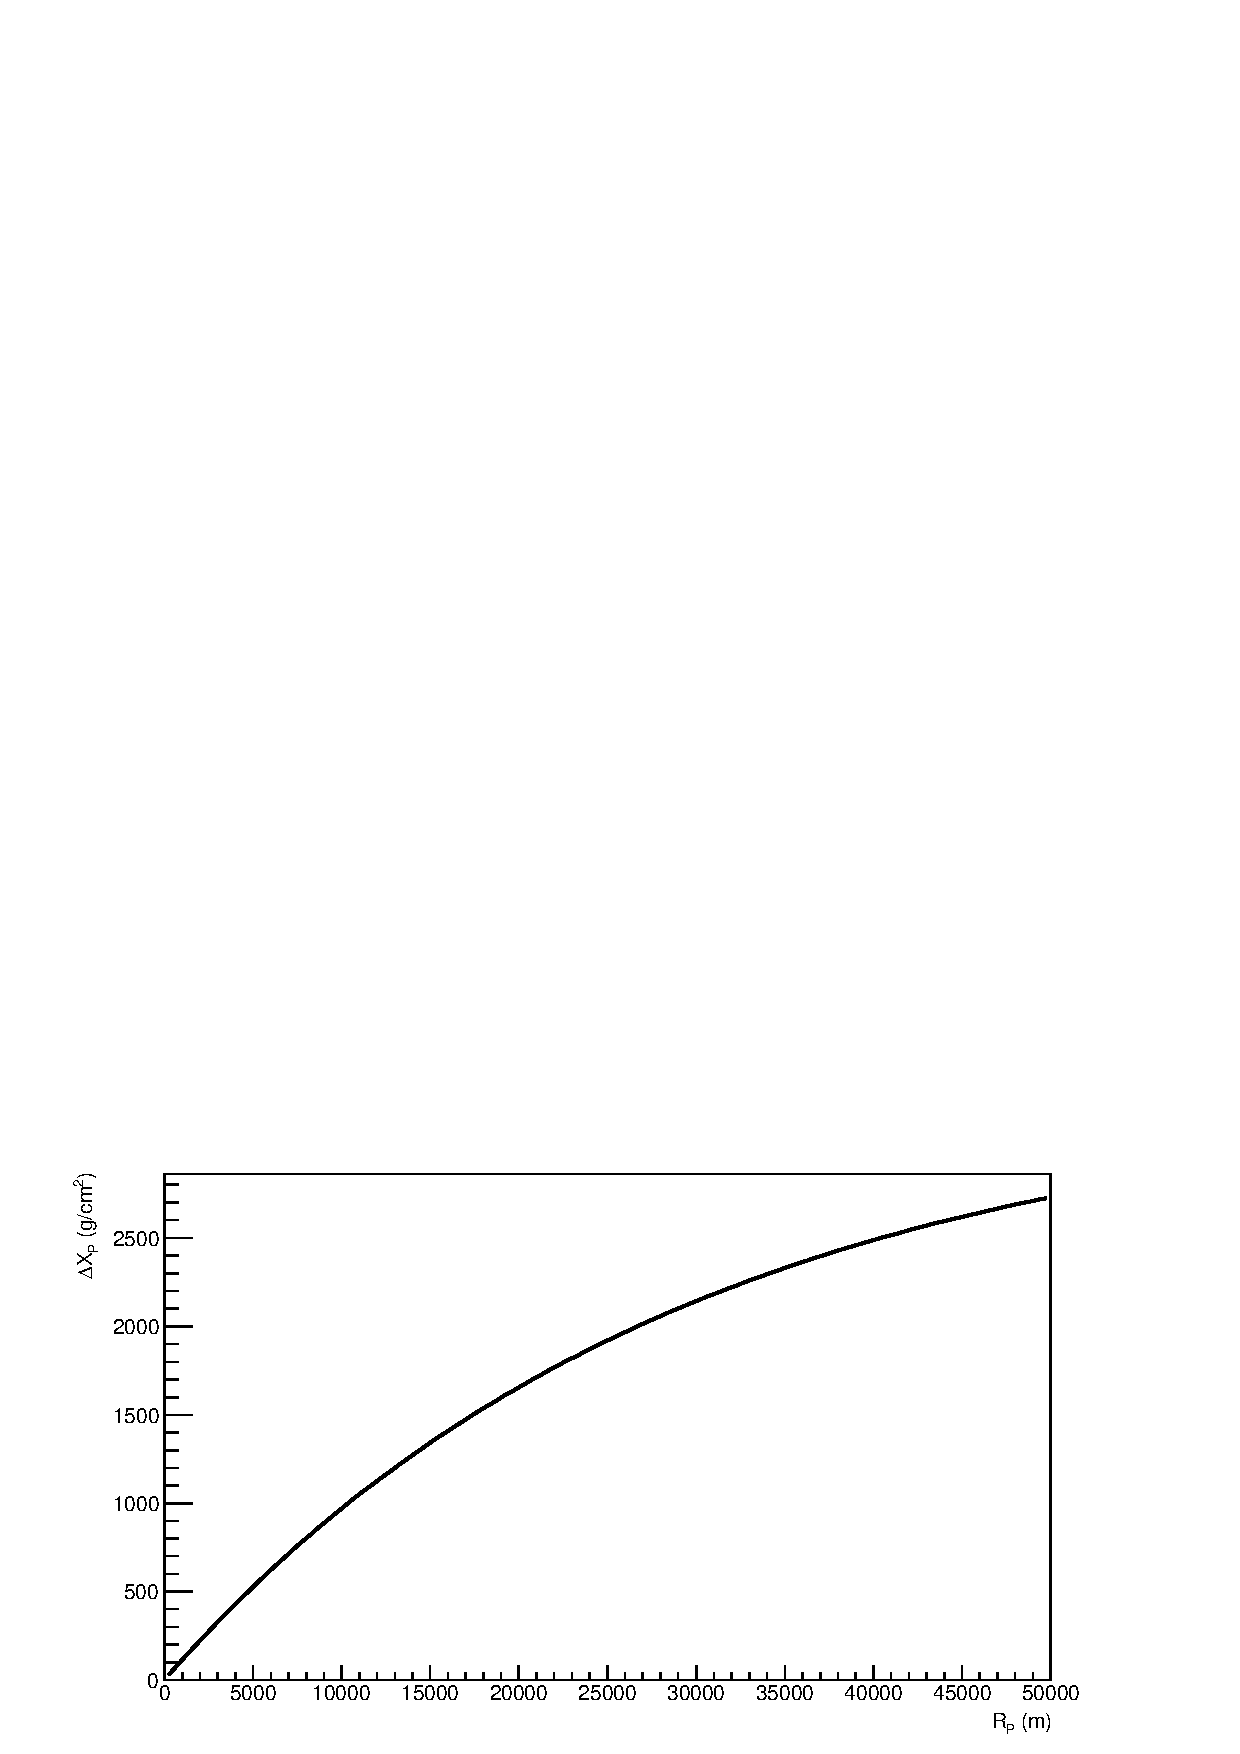
\includegraphics[width=\textwidth]{chapters/graphs/SelectionEff/XpVsRp.pdf}
\caption{How the relationship between the distance to the shower axis and grammage along the path. In this case the distance to the shower axis is denoted R$_P$ and the grammage is denoted $\Delta$X$_P$. The angle of the shower is 15$^{\circ}$}
\end{figure}

\begin{figure}
\centering
\includegraphics[width=\textwidth]{chapters/graphs/SelectionEff/RangeIncreaseVsRangeStand_Xp.pdf}
\caption{The image of how a detector measure the Signal-to-Noise ratio the NSB at the Standard value and Increased by a factor of 10 as a function of distance. The dashed black line denotes the distances where the Signal-to-Noise ratio is the same. The solid black line denotes where the distances are equal.}
\includegraphics[width=\textwidth]{chapters/graphs/SelectionEff/RatioAreaVsDistance_Xp.pdf}
\caption{The image shows how the ratio of the detector viewing area changes with increasing the NSB by a factor of 10 as a function of distance from the detector. The solid black line denotes where the Signal-to-Noise ratio is the same.}
\end{figure}

\begin{figure}
\centering
\begin{subfigure}[b]{0.45\textwidth}
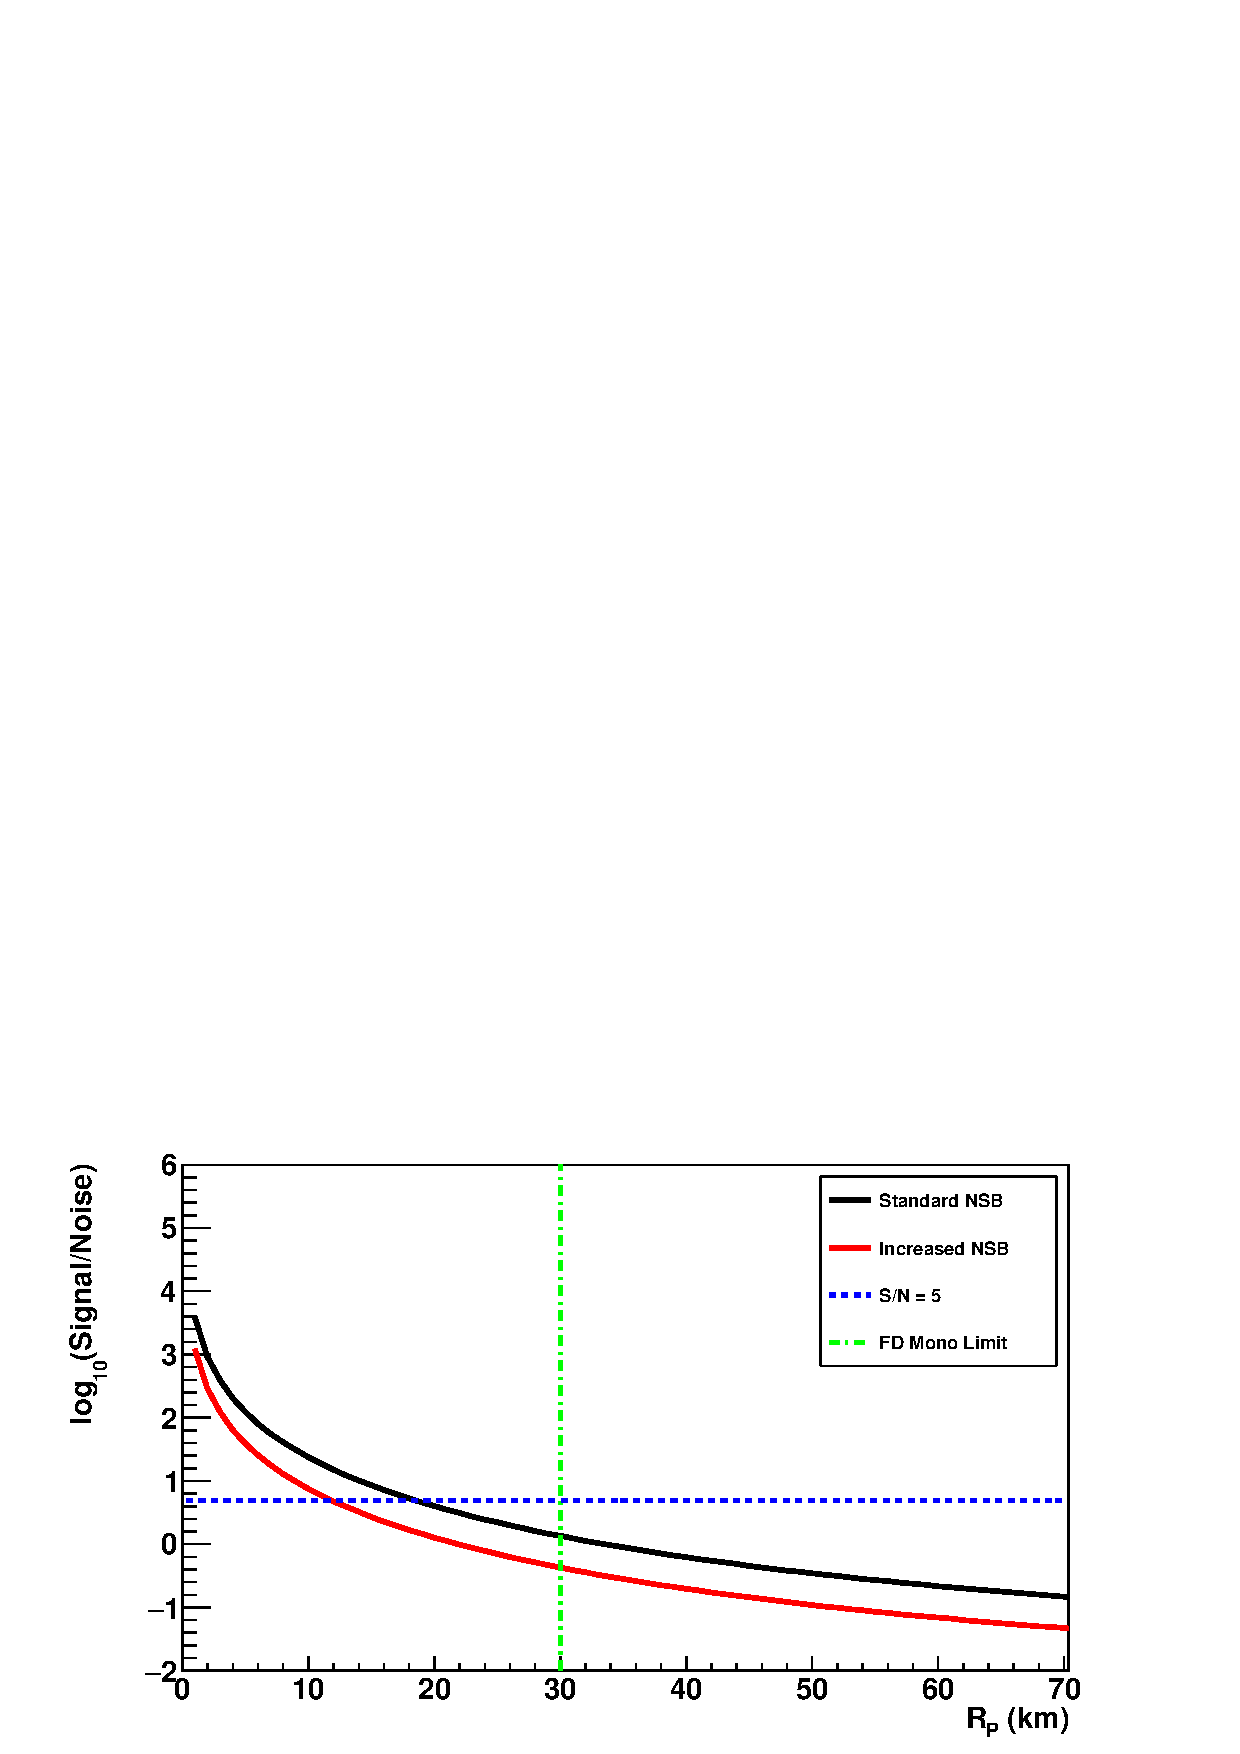
\includegraphics[width=\textwidth]{chapters/graphs/SelectionEff/SignalToNoiseVsDistance_E1e18eV.pdf}
\caption{E = 1 $\times$ 10$^{18}$ eV}
\end{subfigure}
\hspace{3mm}
\begin{subfigure}[b]{0.45\textwidth}
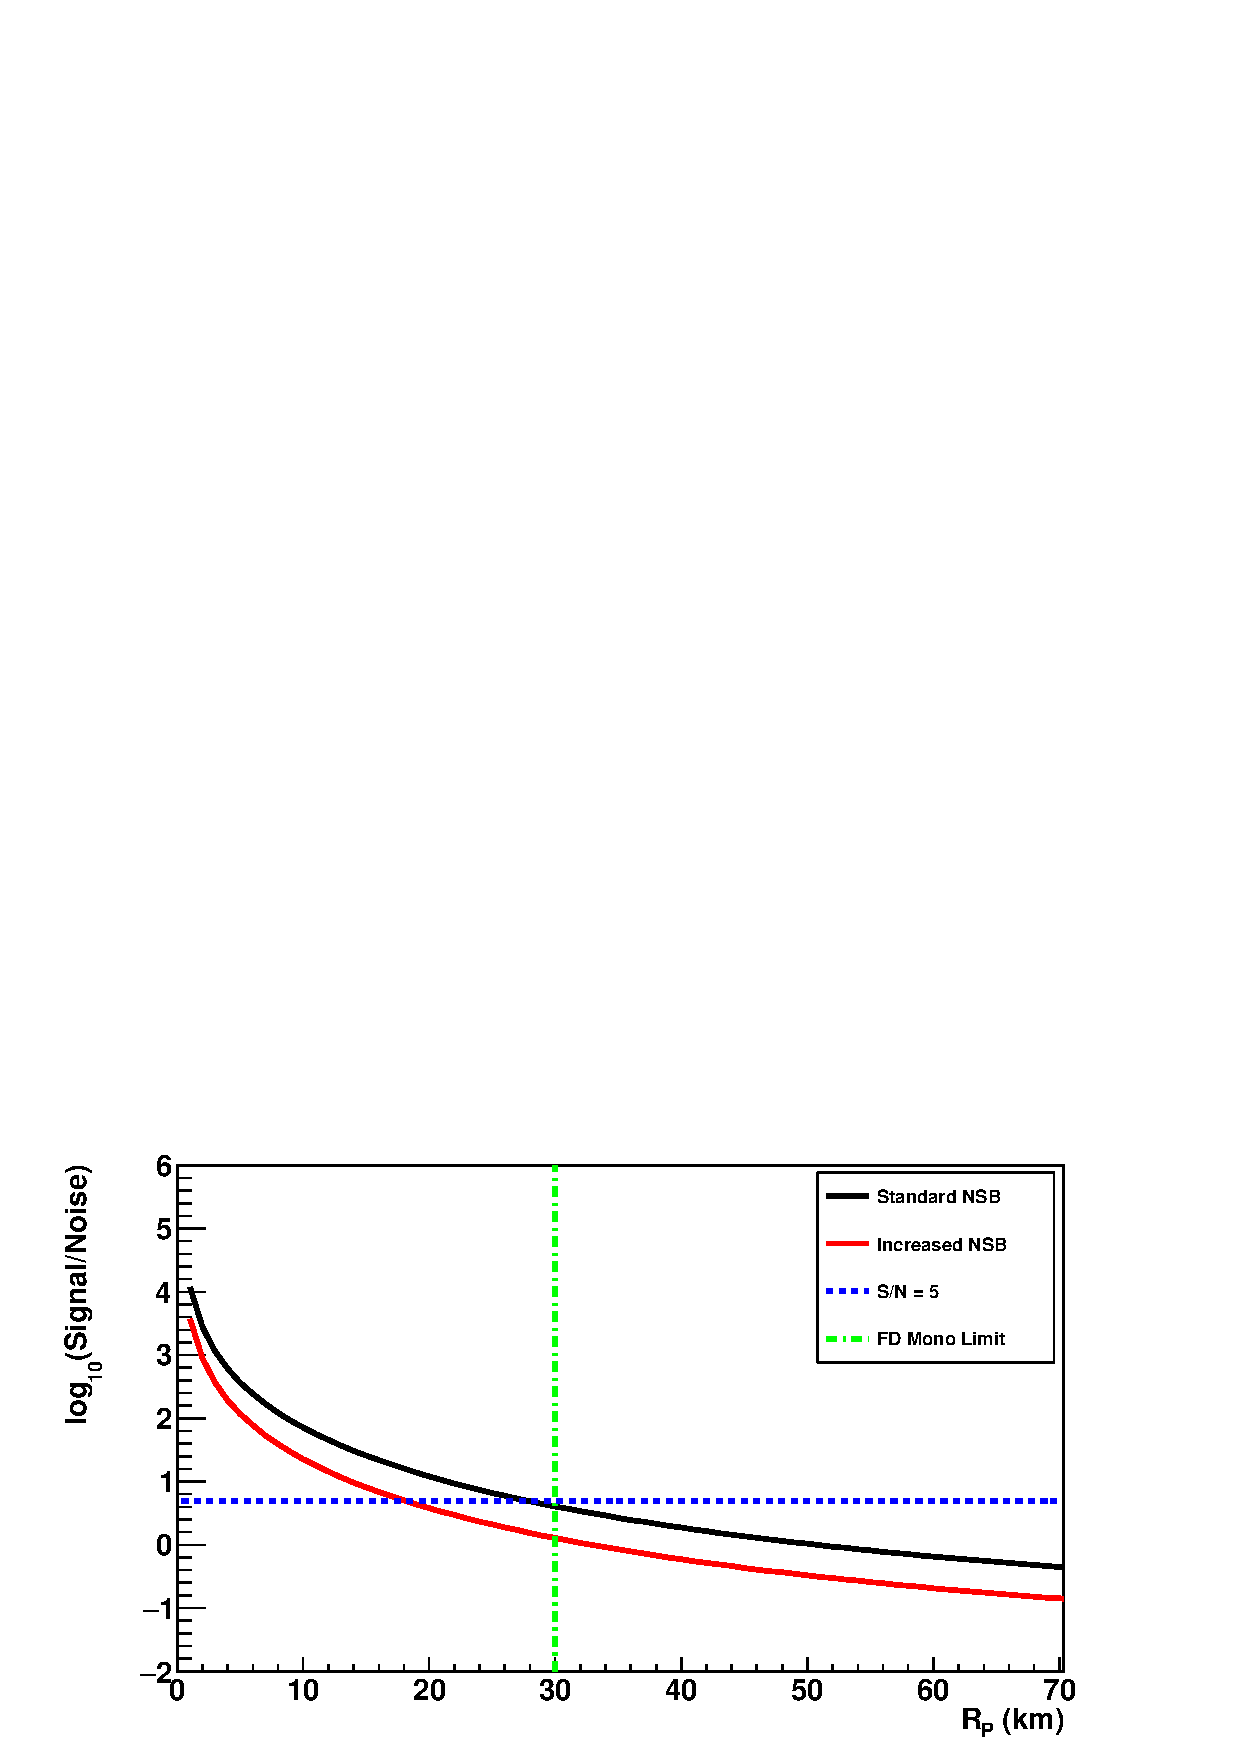
\includegraphics[width=\textwidth]{chapters/graphs/SelectionEff/SignalToNoiseVsDistance_E3e18eV.pdf}
\caption{E = 3 $\times$ 10$^{18}$ eV}
\end{subfigure}
\vspace{3mm}
\begin{subfigure}[b]{0.45\textwidth}
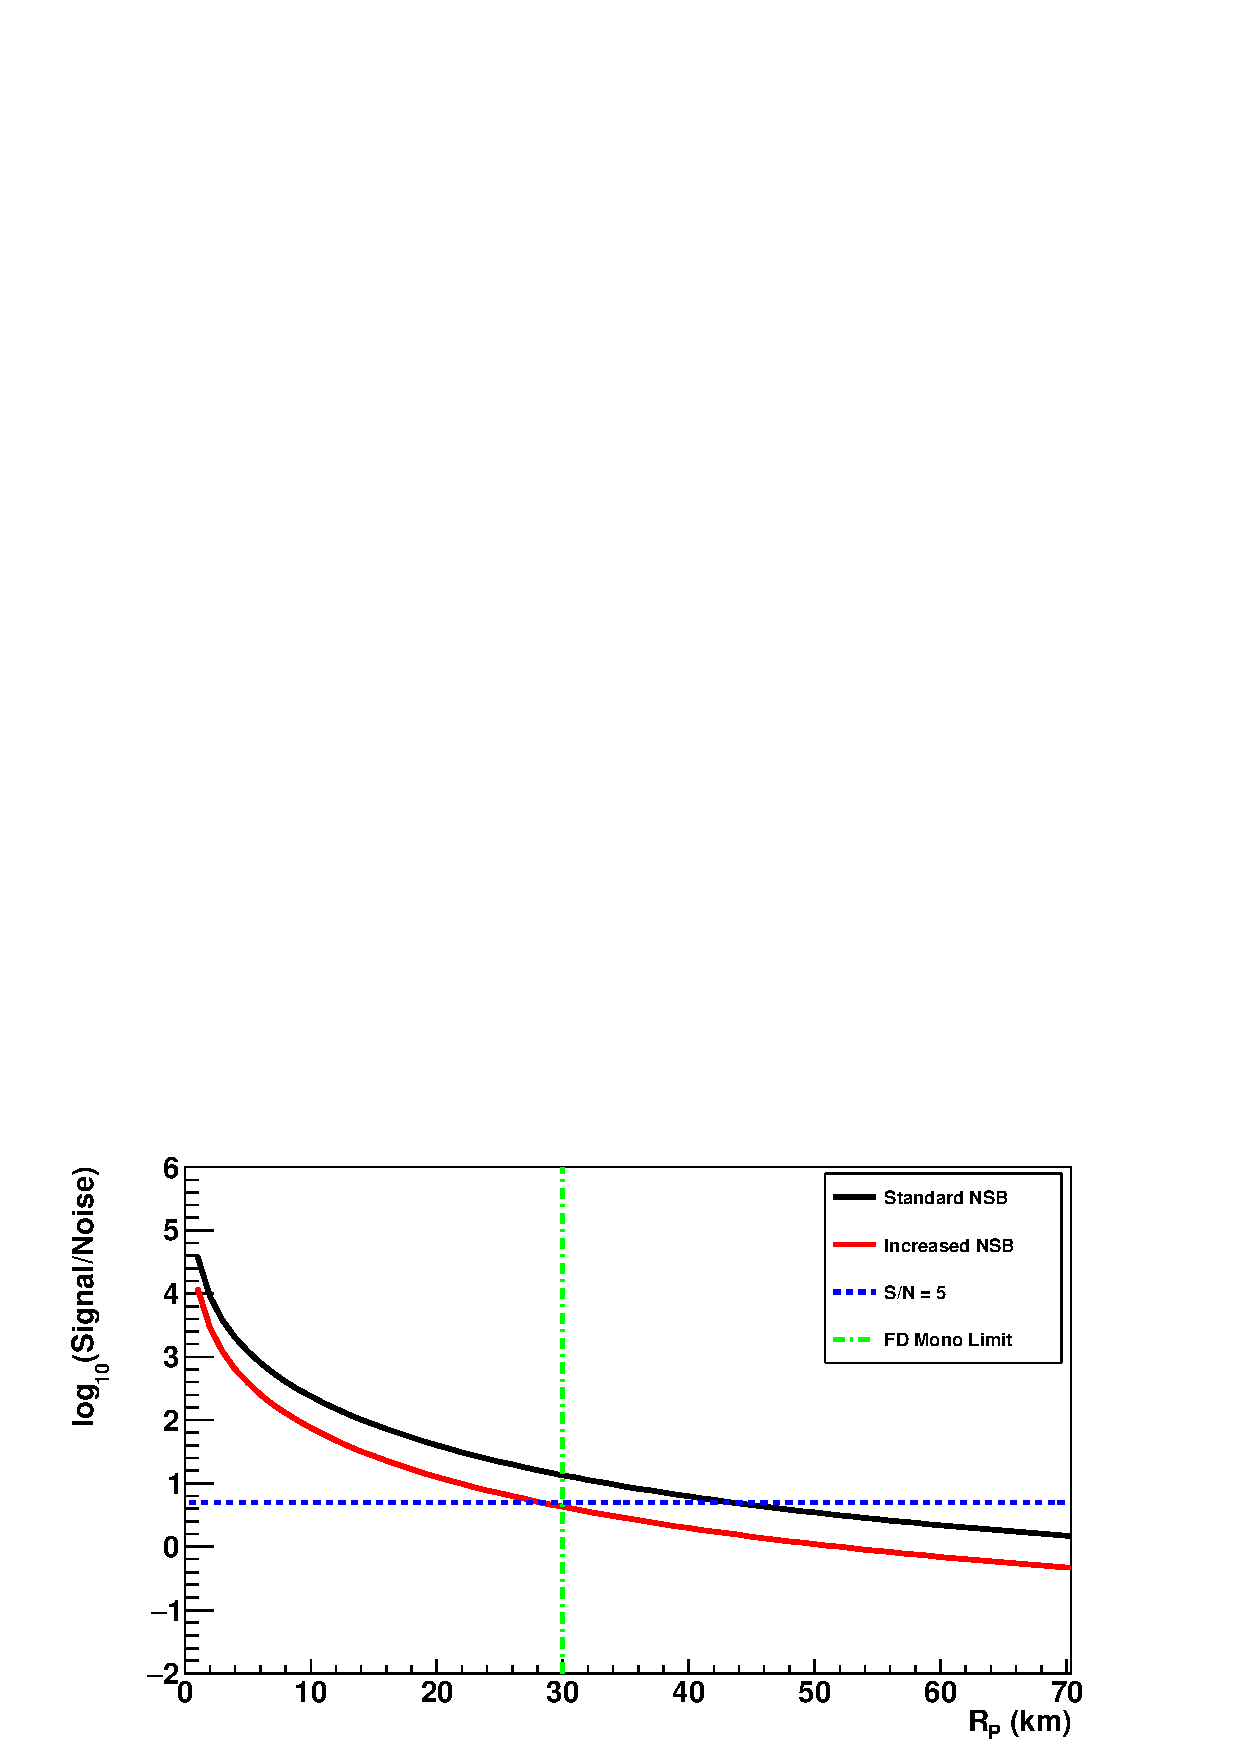
\includegraphics[width=\textwidth]{chapters/graphs/SelectionEff/SignalToNoiseVsDistance_E1e19eV.pdf}
\caption{E = 1 $\times$ 10$^{19}$ eV}
\end{subfigure}
\hspace{3mm}
\begin{subfigure}[b]{0.45\textwidth}
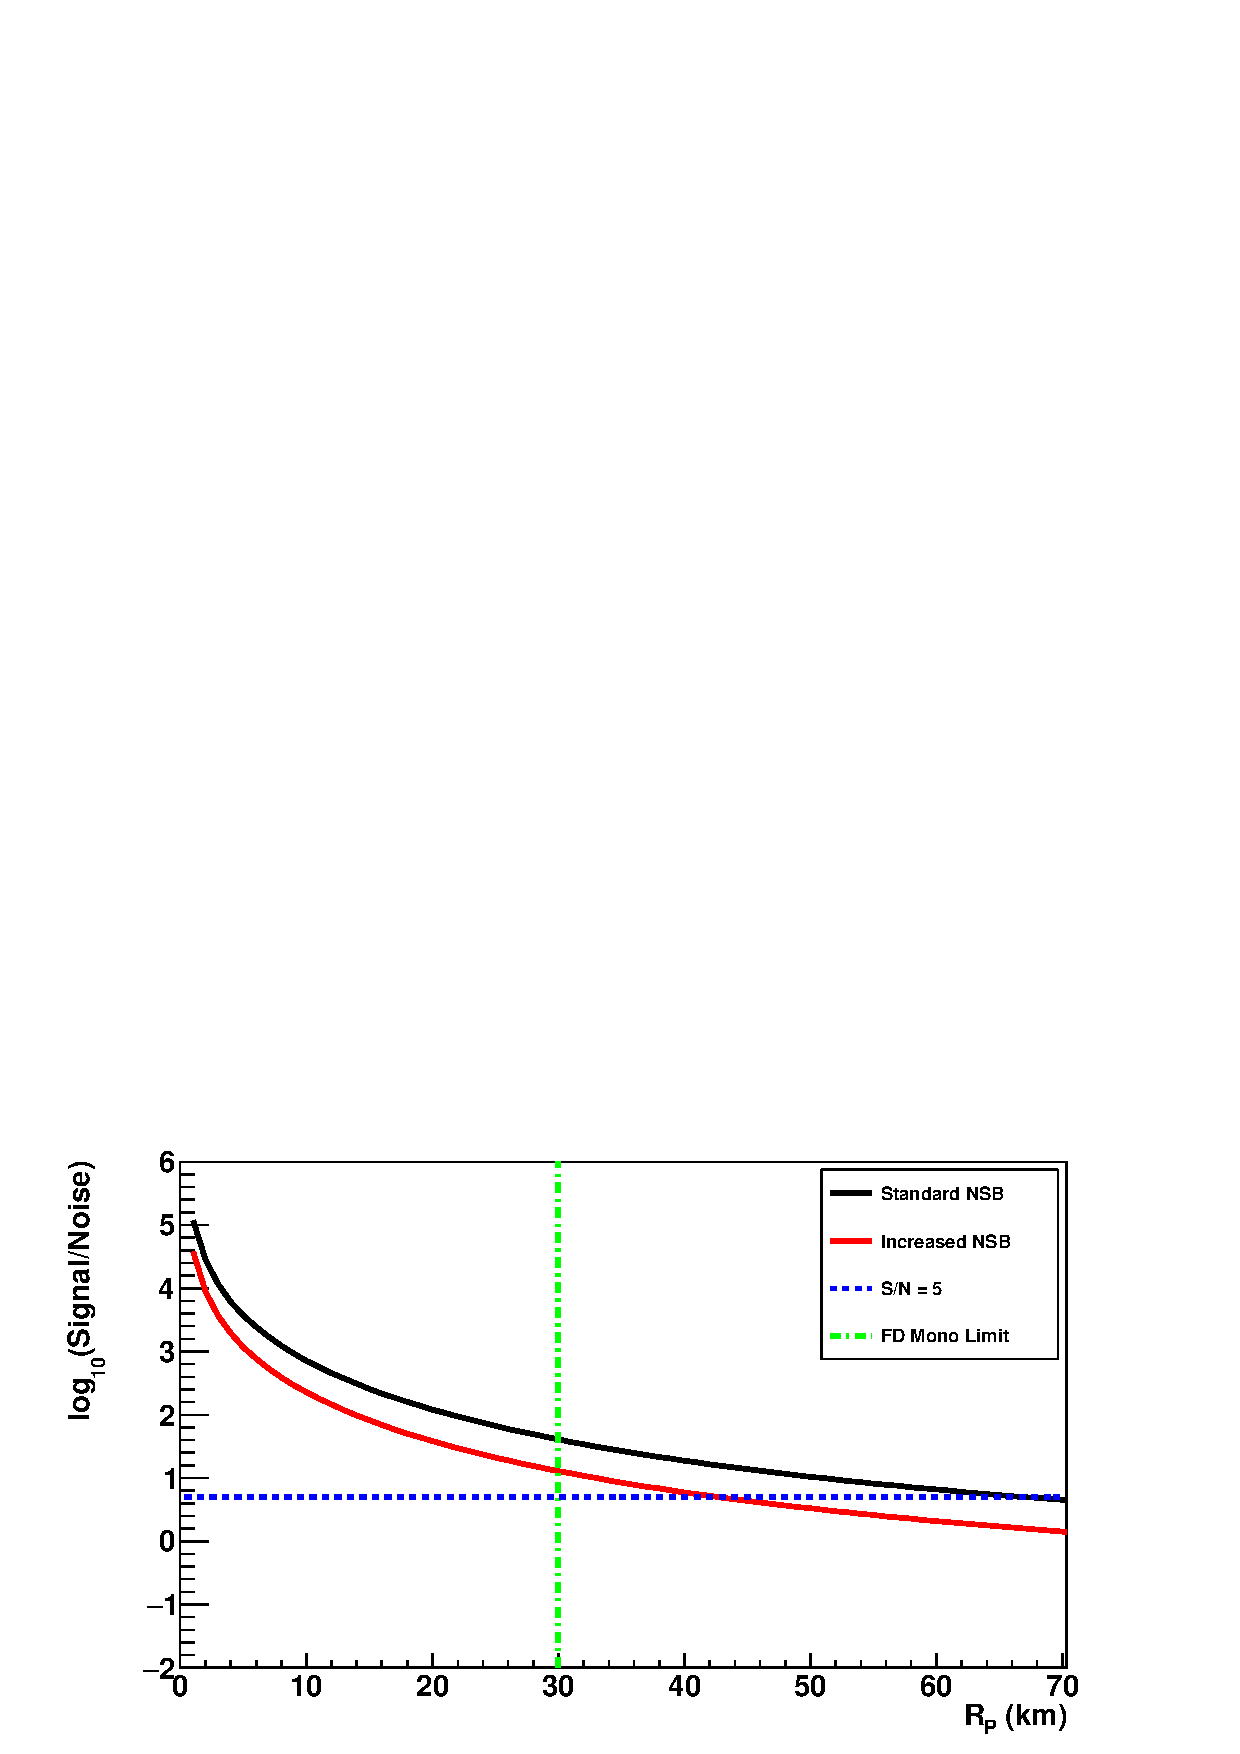
\includegraphics[width=\textwidth]{chapters/graphs/SelectionEff/SignalToNoiseVsDistance_E3e19eV.pdf}
\caption{E = 3 $\times$ 10$^{19}$ eV}
\end{subfigure}
\caption{Using values for the equation to calculate the Signal-to-Noise ratio from specific values for the FD, NSB and conversion's from shower energy to photons to photo-electrons. }
\end{figure}

\section{Increasing NSB in Real Data to evaluate Reconstruction Efficiency}


I investigated evaluating increasing the NSB by different factors on event reconstruction seen by the FD's through two different methods. In this section I will be discussing the method used to evaluate the effects of increasing the NSB on the reconstruction efficiency with the use of real data. The method involved using the raw signal traces from fluorescence telescope EAS shower events that would passed reconstruction and quality cuts and adding addition variance in ADC$^2$ equivalent to an increased NSB from moonlight to the FD pixel signal traces.  The shower events are then reconstructed and passed through the same quality cuts. 

This a repetition of a similar method that M. Unger had preformed in \textbf{2012}. \textbf{Also need to refer to the study done by Brue and Andrew Smith around 1999}. Adding artificial noise to the signal traces was used as an initial proof of concept that EAS showers could still be reconstructed with our current software package. I repeated this study to have a known base-line to work from and have the ability to perform a deeper analysis to understand any underlying mechanics. 

\subsection{Method}
 The Efficiency was calculated with the equation used:
\begin{equation}
\mathrm{Efficiency} = \mathrm{N}^{'}_{\mathrm{Select}} \ / \ \mathrm{N}^0_{\mathrm{Select}}
\end{equation}
where $\mathrm{N}^{0}_{\mathrm{Select}}$ is the number of selected events at the standard NSB level and $\mathrm{N}^{'}_{\mathrm{Select}}$ is the number of selected events at the increased NSB
level. 

After the Efficiency was calculated the bias and resolution for Xmax and energy was determined. For real data, the bias is the relative change in the mean of the distributions at increased NSB to the mean of the distributions at standard NSB, both after reconstruction and selection cuts. The bias calculations for real data become:
\begin{eqnarray}
\Delta \mathrm{E}_{\mathrm{Data}} &=& \frac{\mathrm{E}_{\mathrm{IncreasedNSB}} - \mathrm{E}_{\mathrm{StandardNSB}}}{\mathrm{E}_{\mathrm{StandardNSB}}} \label{eq:energybias_data} \\
\Delta \mathrm{Xmax}_{\mathrm{Data}} &=& \mathrm{Xmax}_{\mathrm{IncreasedNSB}} - \mathrm{Xmax}_{\mathrm{StandardNSB}}\label{eq:xmaxbias_data}
\end{eqnarray} 
For simulated data the bias is the relative change in the mean of the distributions after the full simulation by EAS events going through an atmosphere with a specified NSB photon field, the FD telescopes optics, trigger, reconstruction and selection cuts compared with Monte-Carlo truth.
\begin{eqnarray}
\Delta \mathrm{E}_{\mathrm{Sim}} &=& \frac{\mathrm{E}_{\mathrm{recon}} - \mathrm{E}_{\mathrm{true}}}{\mathrm{E}_{\mathrm{true}}}  \label{eq:energybias_sim} \\
\Delta \mathrm{Xmax}_{\mathrm{Sim}} &=& \mathrm{Xmax}_{\mathrm{recon}} - \mathrm{Xmax}_{\mathrm{true}} \label{eq:xmaxbias_sim}
\end{eqnarray}
 
 
The energy and Xmax resolution is calculated via:
\begin{eqnarray}
\sigma_{\mathrm{res}} &=& \left( \frac{1}{\mathrm{N}} \sum \frac{1}{\sigma^2_i} \right)^{1/2}
\end{eqnarray}

To further evaluate the effects of increasing the NSB on the quality of the reconstructed EAS data, I look at the resolution and bias of both the reconstructed energy and reconstructed Xmax. A quick reminder that Xmax is the measurement of the brightest part of the shower relating to the maximum number of particles produced. For the smearing method the energy and Xmax bias is comparing to the measured data taken at standard NSB levels to the reconstructed with the increased NSB levels. For the simulations the energy and Xmax bias can be calculated using the true energy and Xmax values used to generate each EAS profile.

The trend of the energy resolution for both methods is that as the energy of the EAS event increases the bias decreases. This was expected as the energy of the shower increases the brighter and longer the track that is observed. A brighter and longer track allows for a better reconstruction.

\subsection{Results}
\begin{figure}
\centering
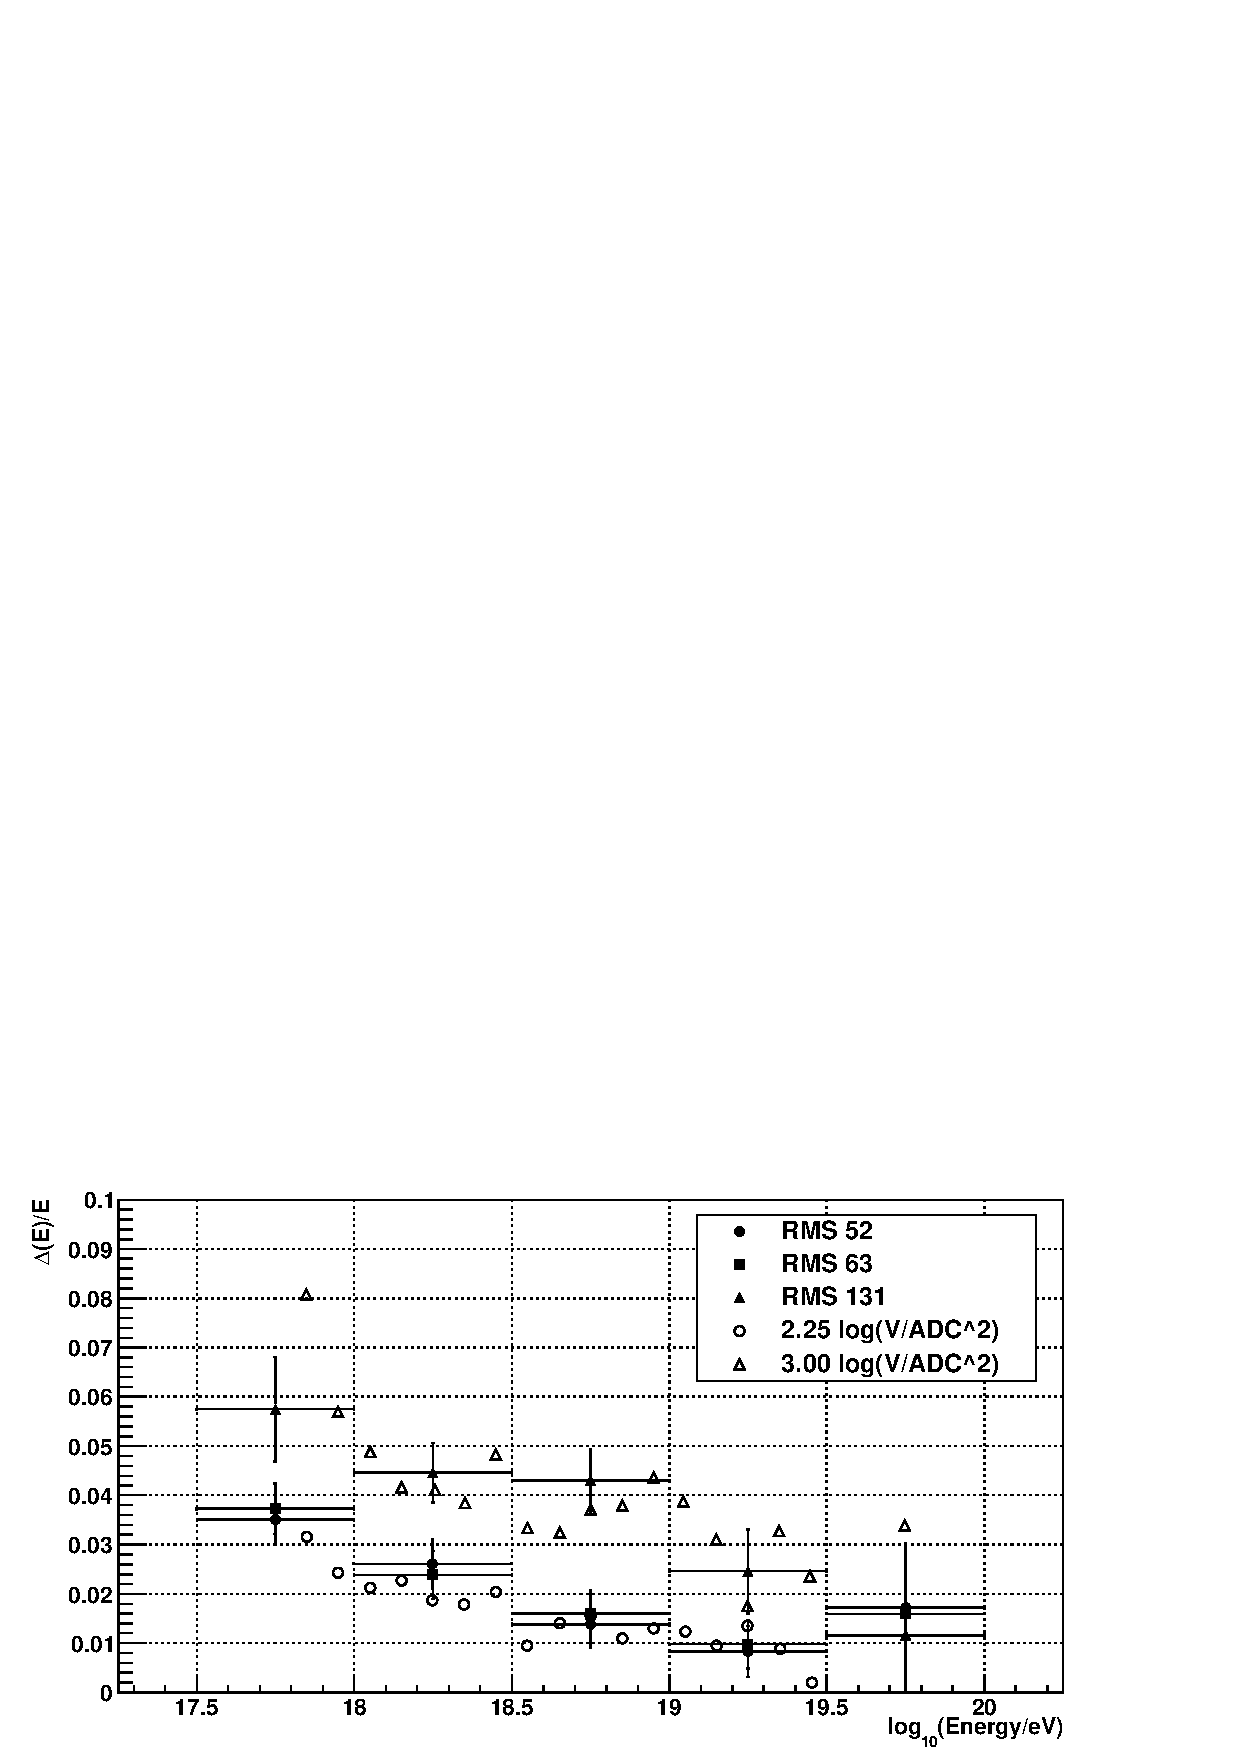
\includegraphics[width=\textwidth]{chapters/graphs/SelectionEff/Smearing_RealData_EnergyBias.pdf}
\caption{Energy Bias using Smearing Method.}
\vspace{3mm}
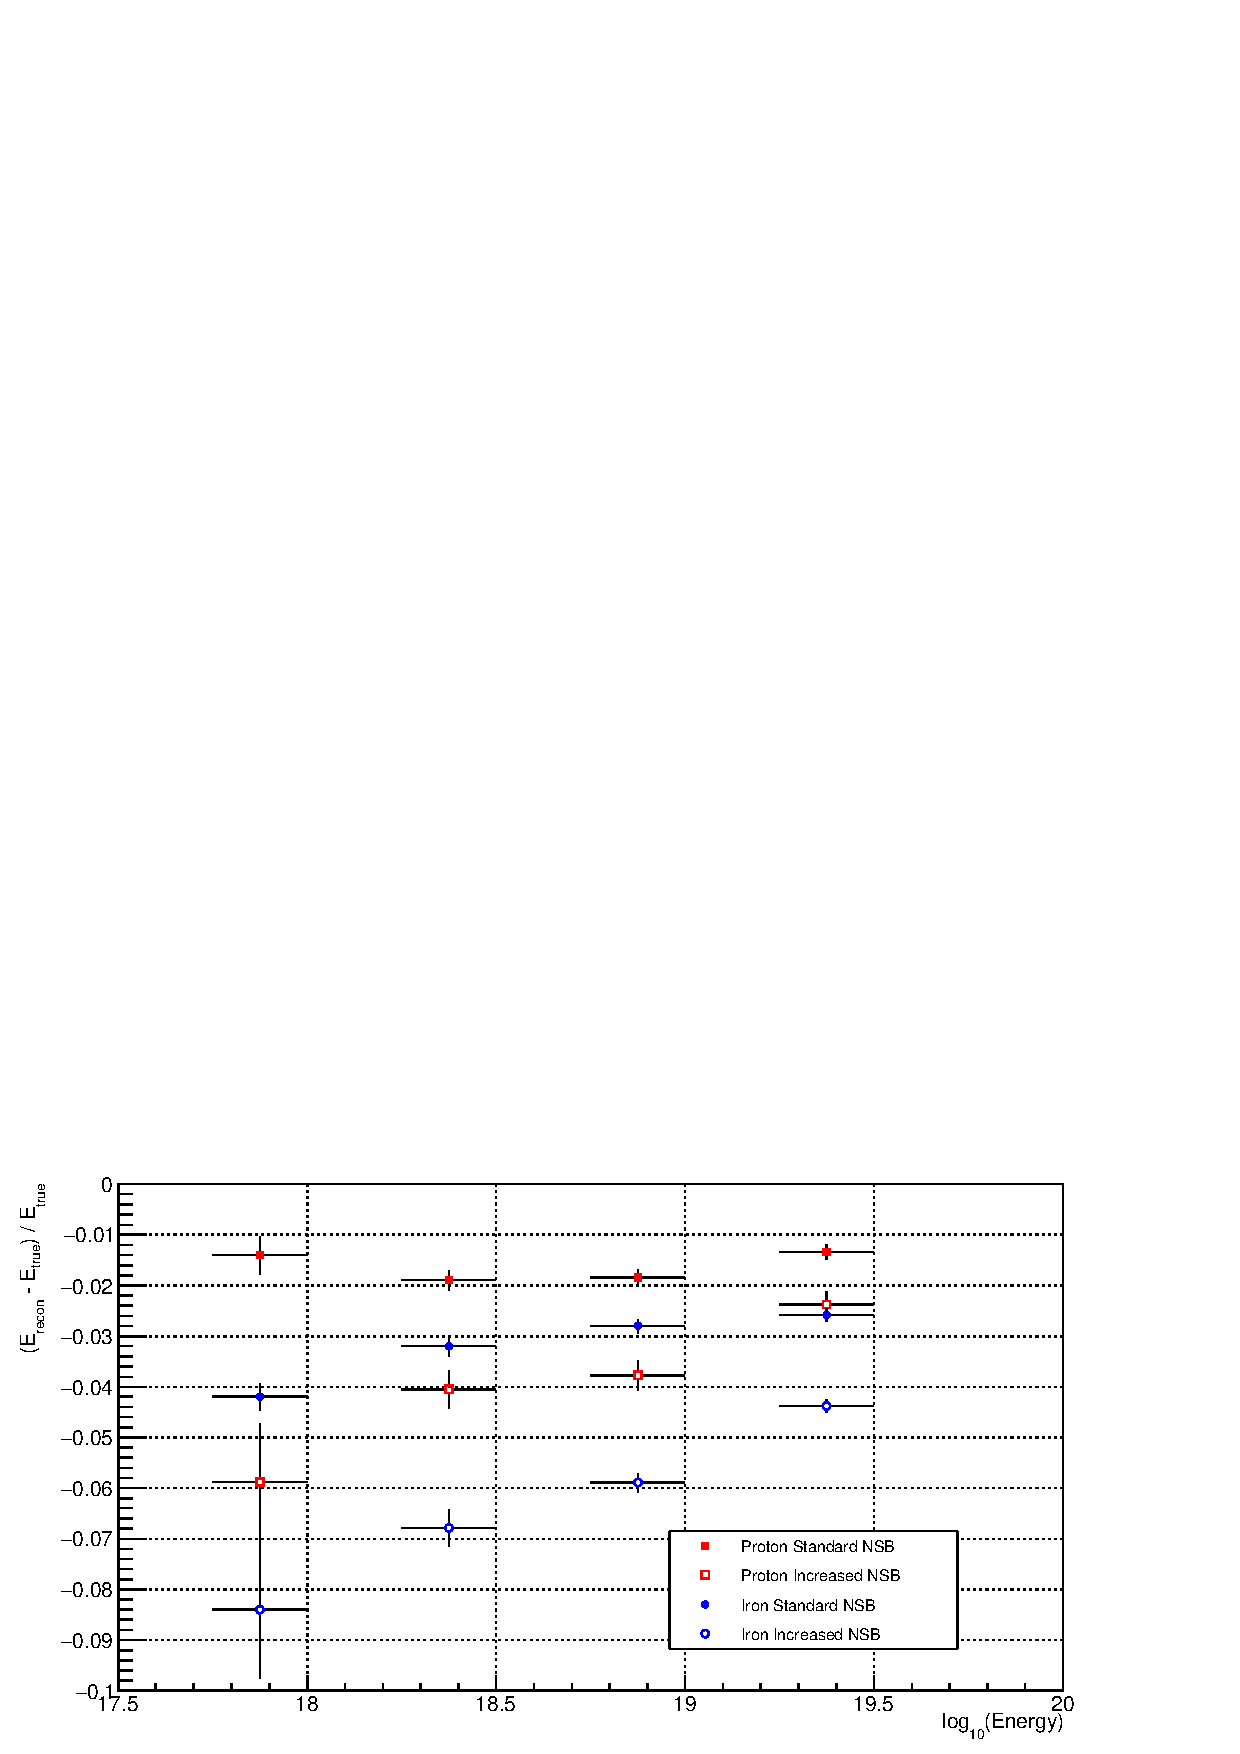
\includegraphics[width=\textwidth]{chapters/graphs/SelectionEff/Simulation_ProtonIron_EnergyBias.pdf}
\caption{Energy Bias using simulated data.}
\end{figure}

\begin{figure}
\centering
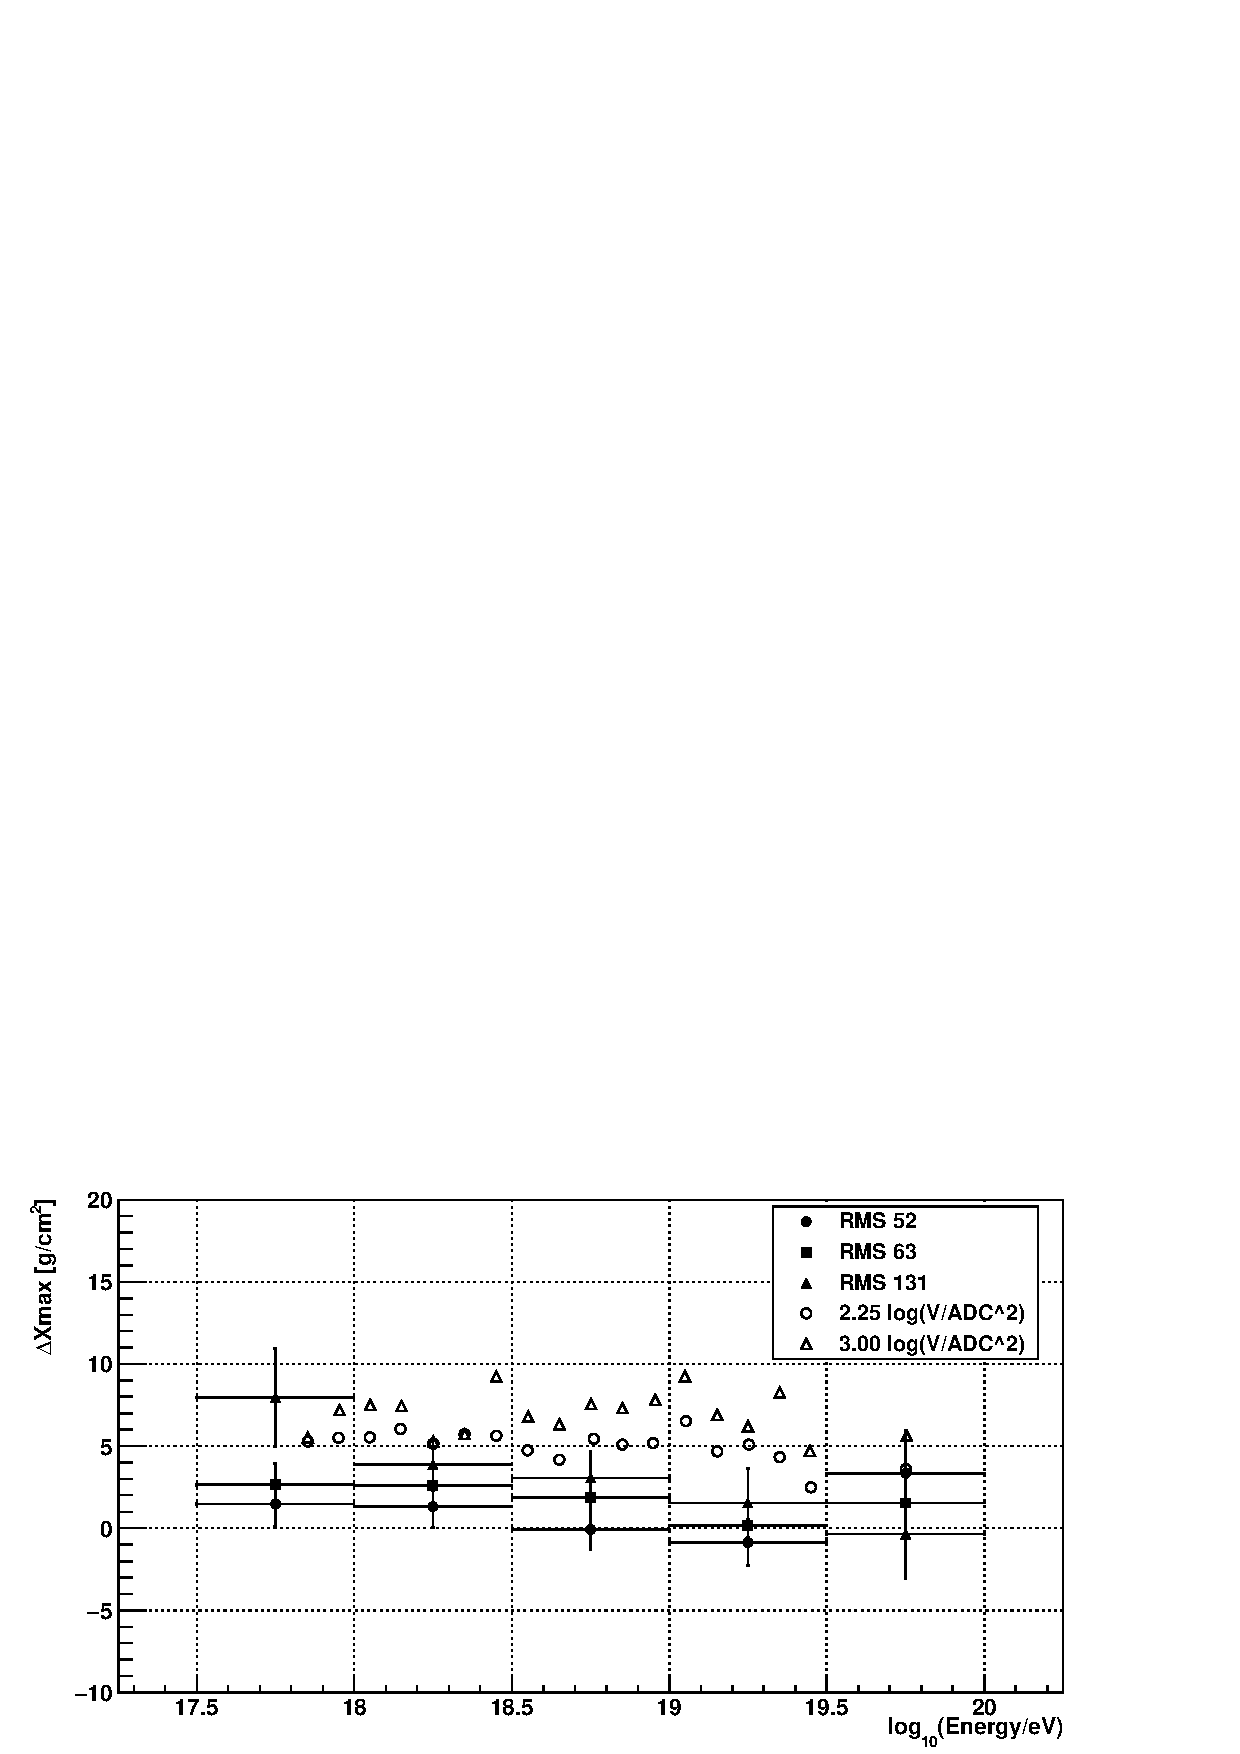
\includegraphics[width=\textwidth]{chapters/graphs/SelectionEff/Smearing_RealData_XmaxBias.pdf}
\caption{Xmax Bias using Smearing Method.}
\vspace{3mm}
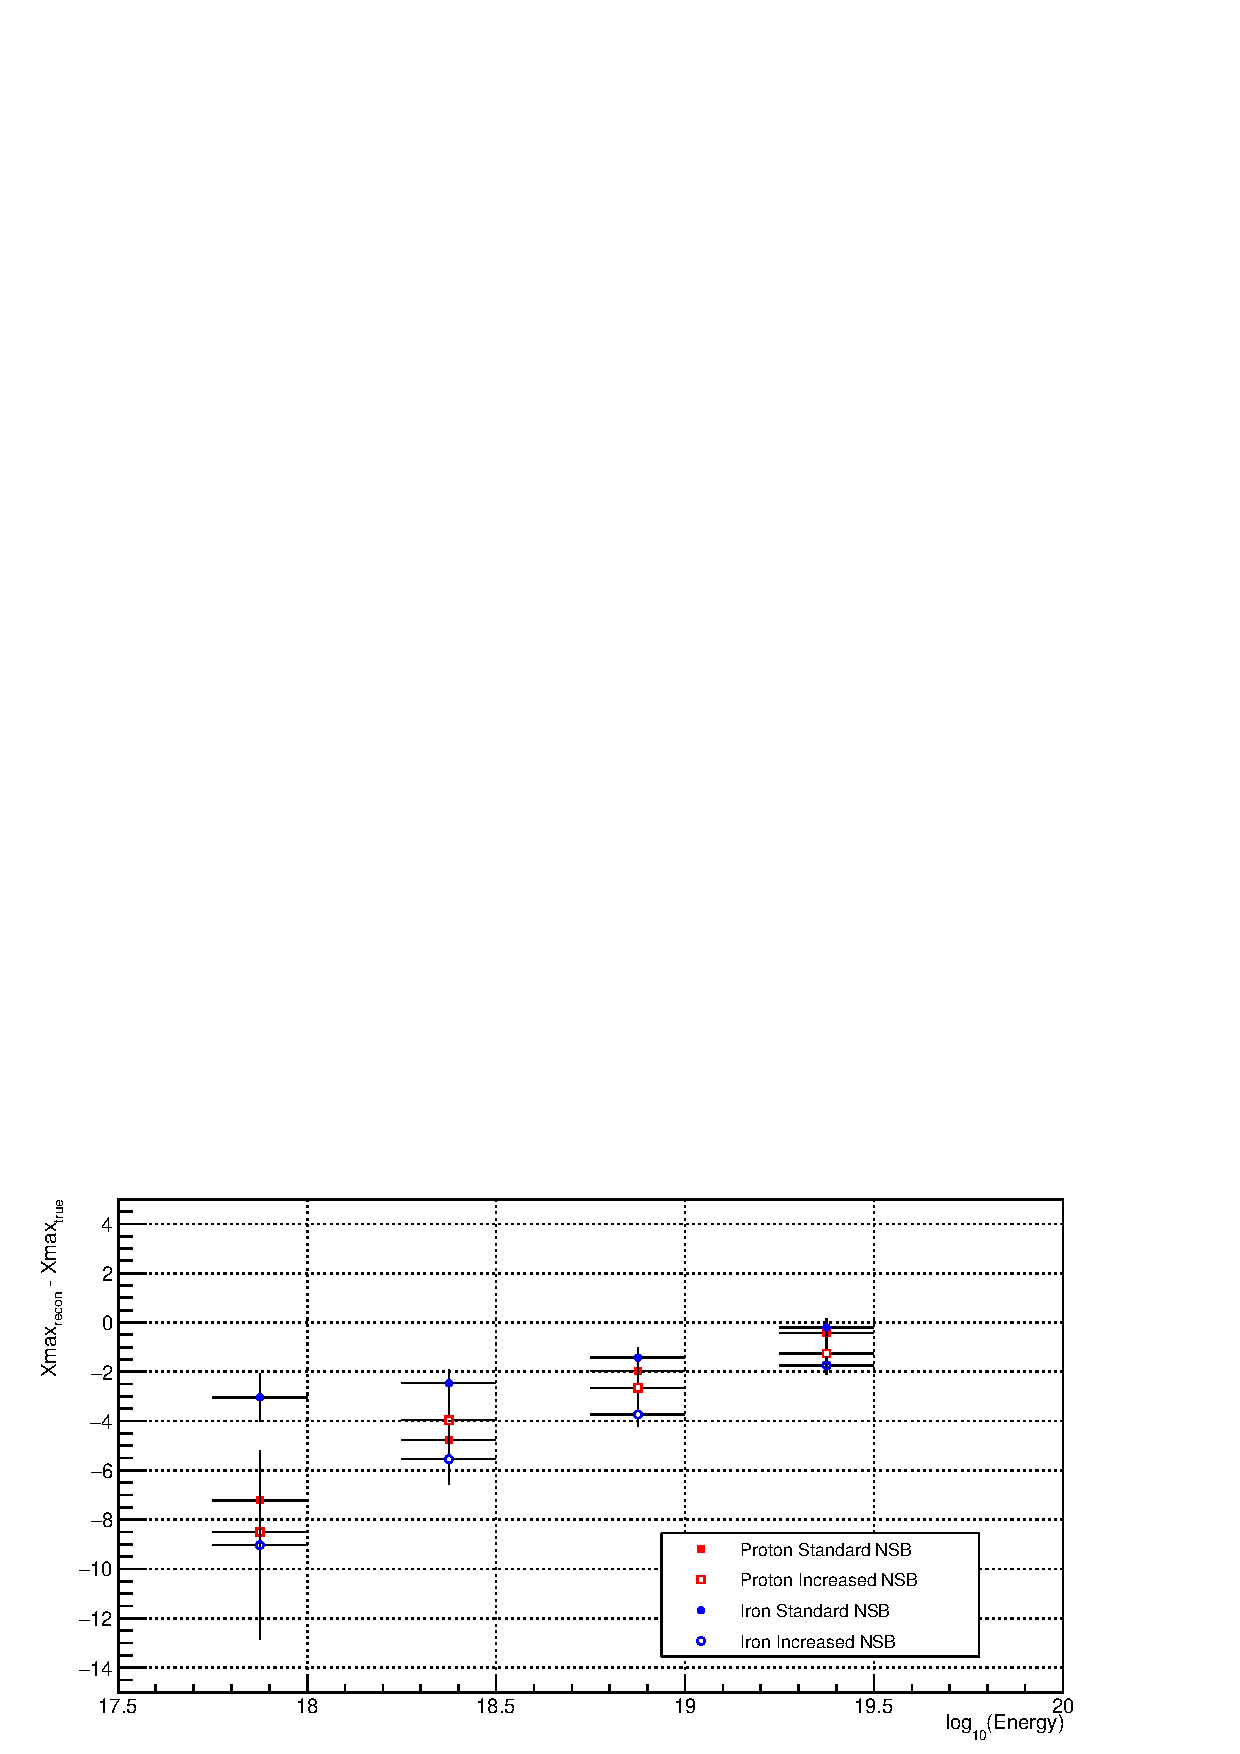
\includegraphics[width=\textwidth]{chapters/graphs/SelectionEff/Simulation_ProtonIron_XmaxBias.pdf}
\caption{Xmax Bias using simulated data.}
\end{figure}

\begin{figure}
\centering
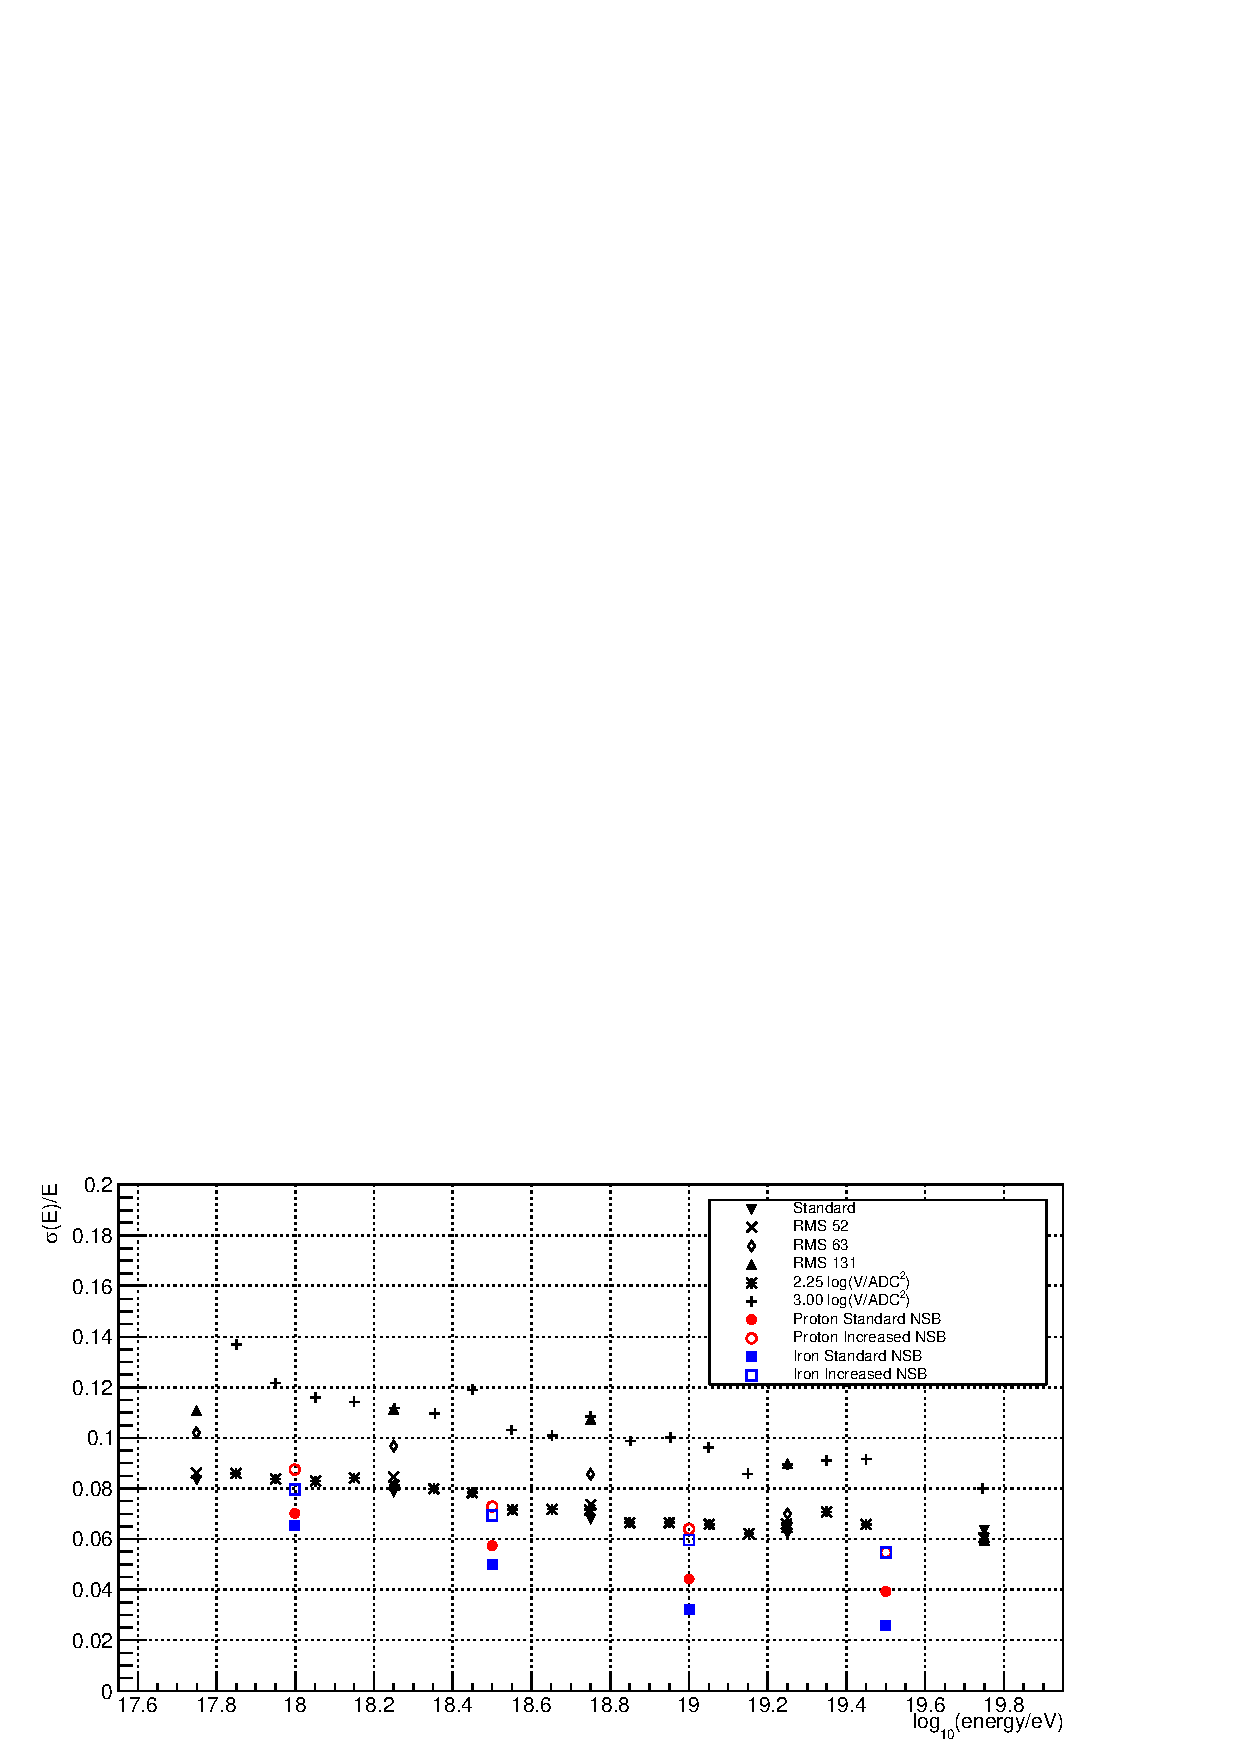
\includegraphics[width=\textwidth]{chapters/graphs/SelectionEff/Combined_EnergyRes_All.pdf}
\caption{Energy Resolution using both Smearing Method data and simulated showers.}
\vspace{3mm}
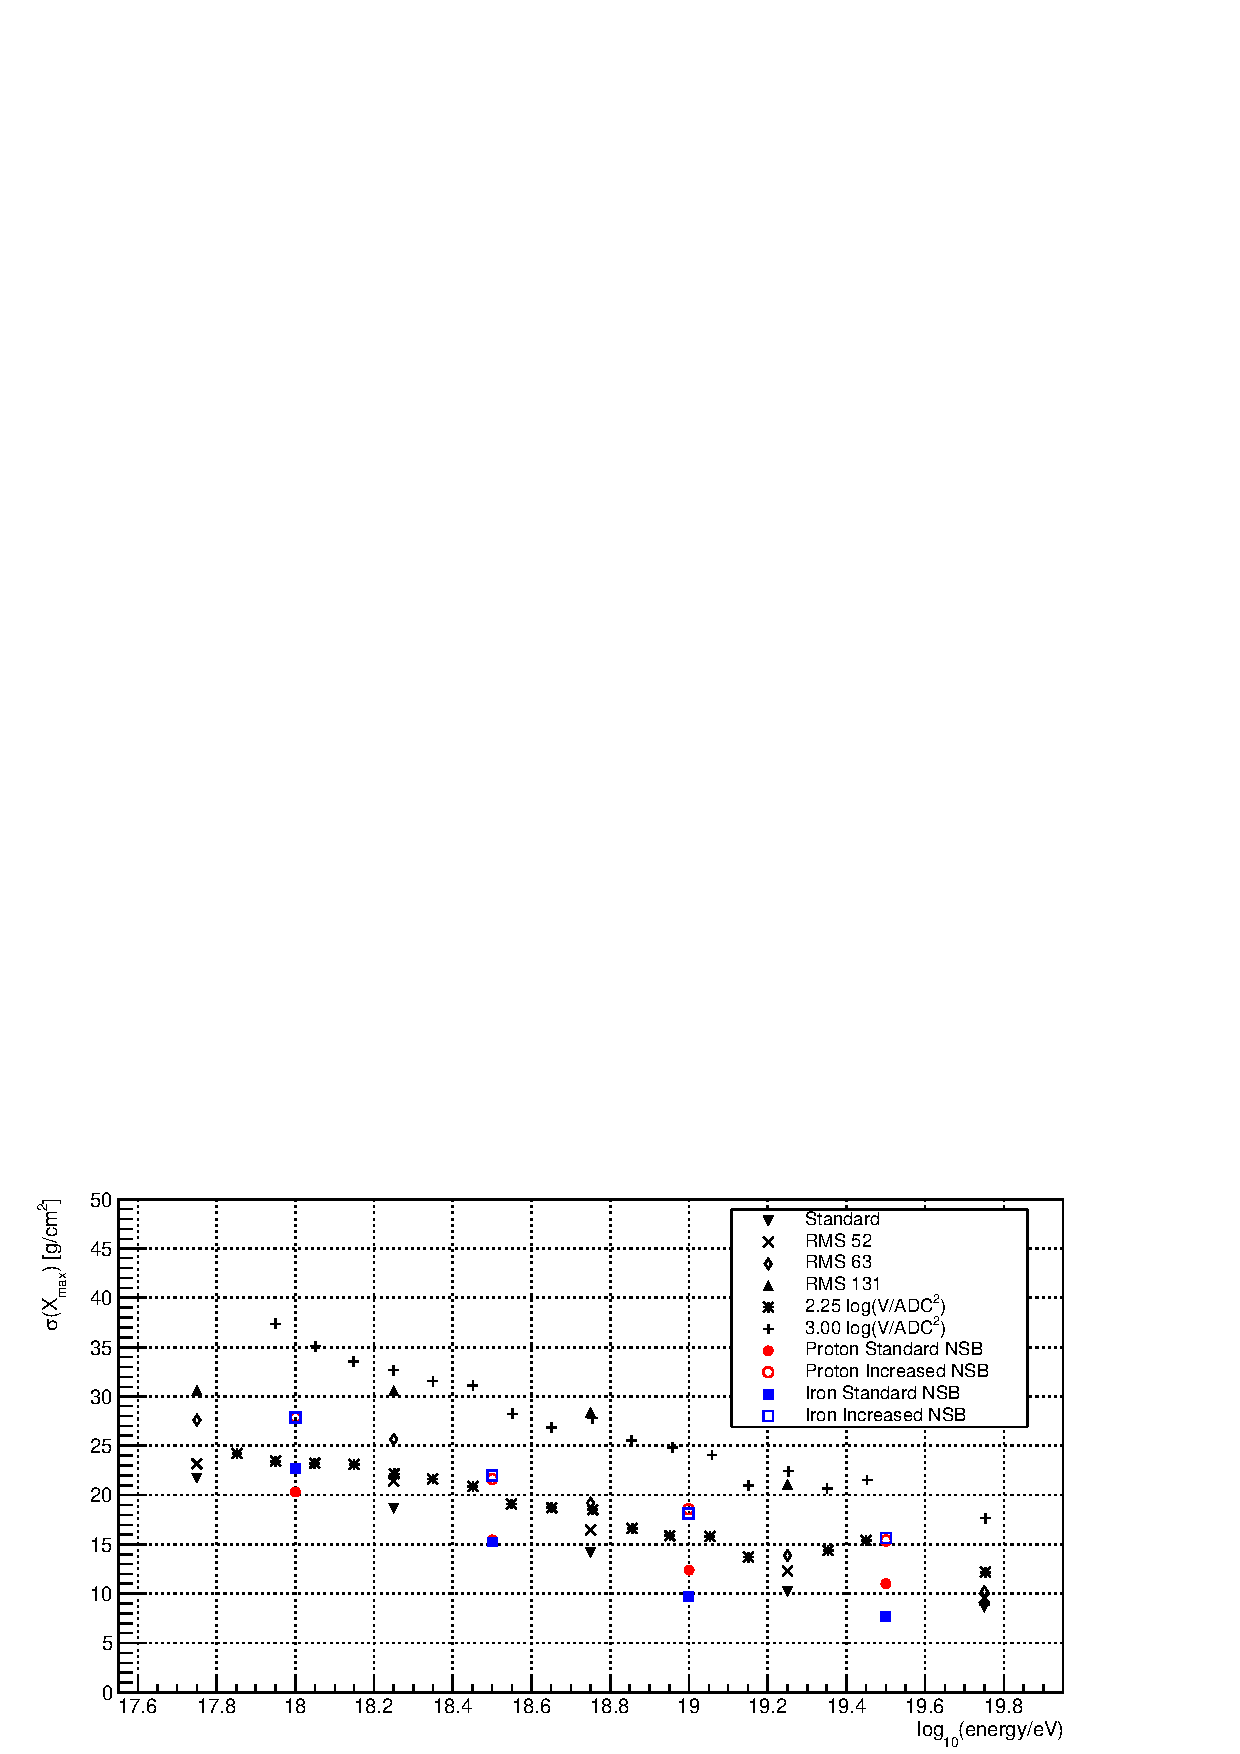
\includegraphics[width=\textwidth]{chapters/graphs/SelectionEff/Combined_XmaxRes_All.pdf}
\caption{Xmax Resolution using both Smearing Method data and simulated showers.}
\end{figure}

\begin{figure}
\centering
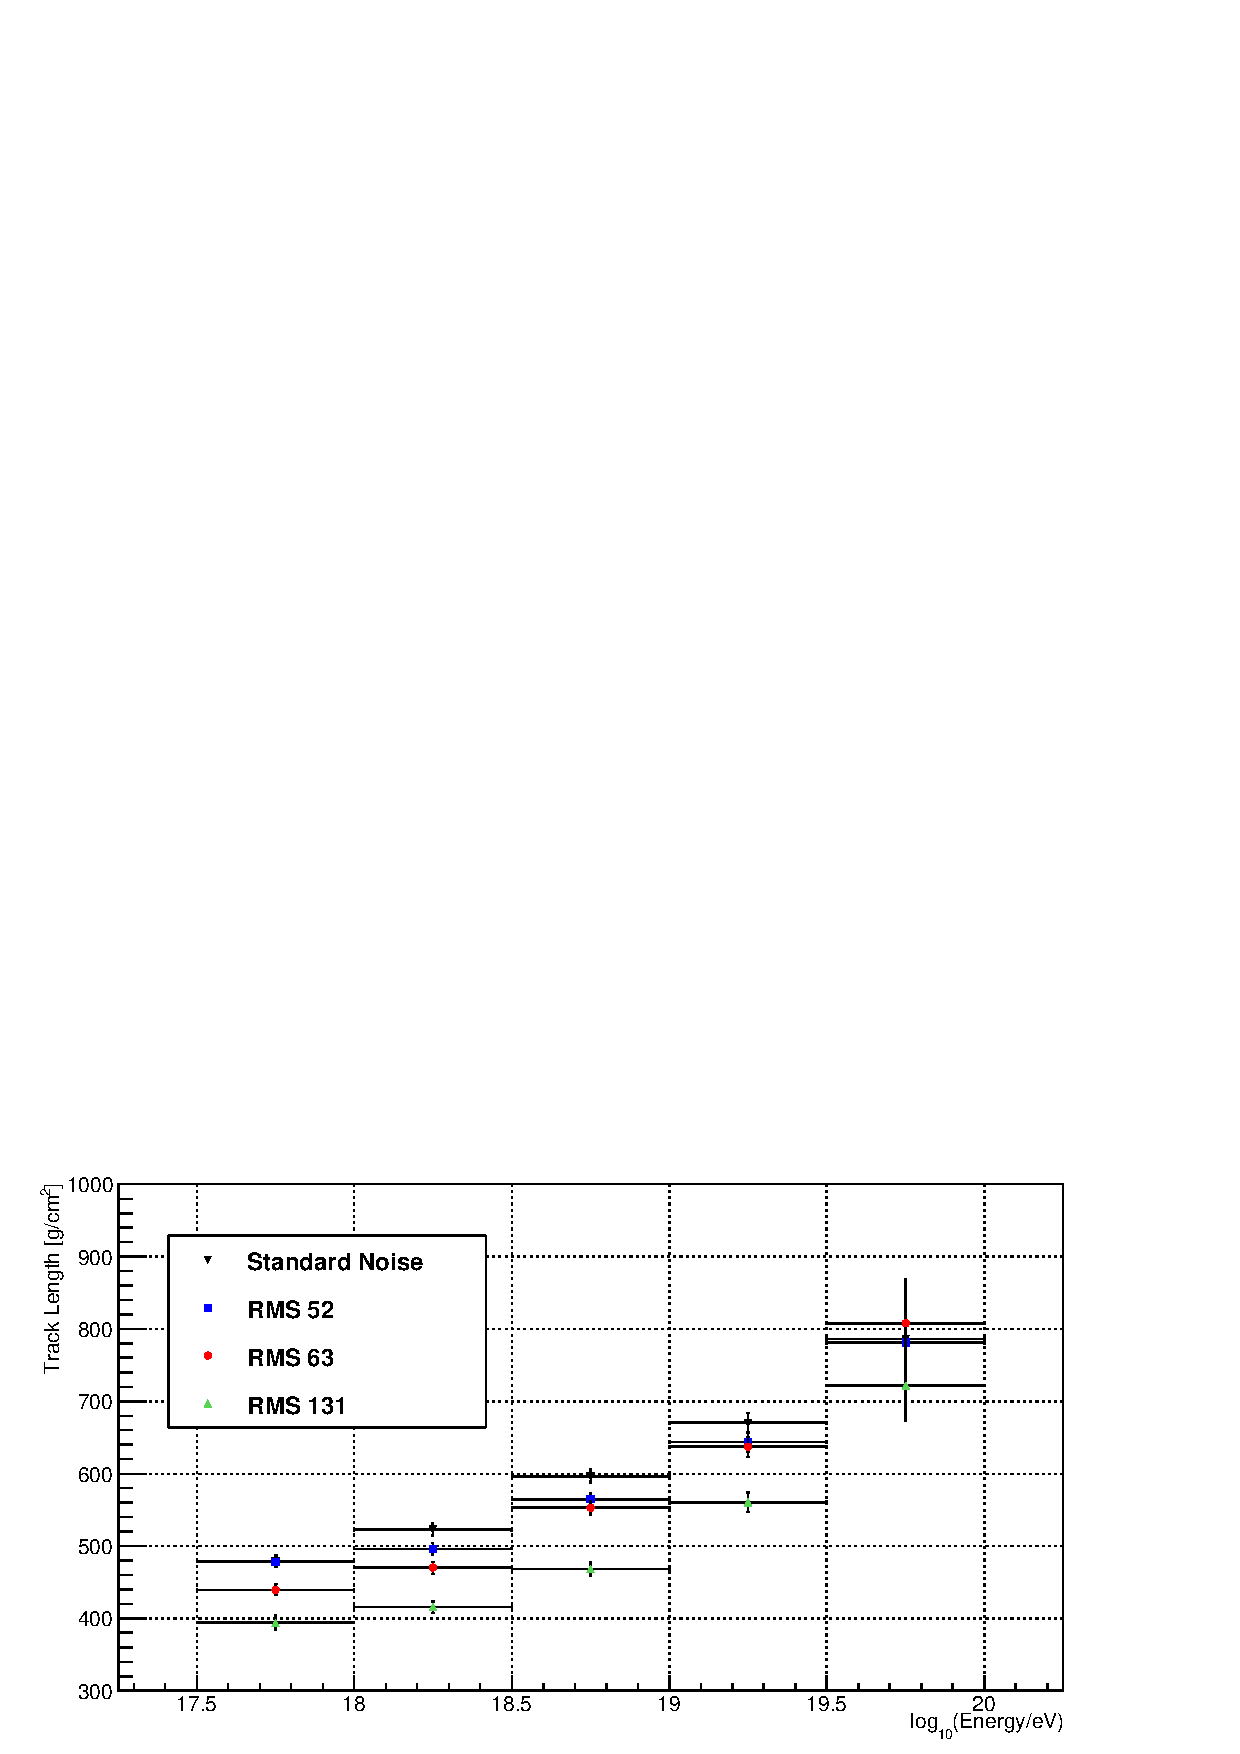
\includegraphics[width=\textwidth]{chapters/graphs/SelectionEff/Smearing_TrackLength_DiffNSBlevels.pdf}
\caption{Track length using Smearing method.} \label{fig:TrackLength_Smearing}
\end{figure}
\subsection{Discussion}

\section{Increasing NSB in Simulations to evaluate Trigger/Reconstruction Efficiency}

\subsection{Method}
 The Efficiency was calculated with the equation used:
\begin{equation}
\mathrm{Efficiency} = \mathrm{N}^{'}_{\mathrm{Select}} \ / \ \mathrm{N}^0_{\mathrm{Select}}
\end{equation}
where $\mathrm{N}^{0}_{\mathrm{Select}}$ is the number of selected events at the standard NSB level and $\mathrm{N}^{'}_{\mathrm{Select}}$ is the number of selected events at the increased NSB
level. 

After the Efficiency was calculated the bias and resolution for Xmax and energy was determined. For real data, the bias is the relative change in the mean of the distributions at increased NSB to the mean of the distributions at standard NSB, both after reconstruction and selection cuts. The bias calculations for real data become:
\begin{eqnarray}
\Delta \mathrm{E}_{\mathrm{Data}} &=& \frac{\mathrm{E}_{\mathrm{IncreasedNSB}} - \mathrm{E}_{\mathrm{StandardNSB}}}{\mathrm{E}_{\mathrm{StandardNSB}}} \label{eq:energybias_data} \\
\Delta \mathrm{Xmax}_{\mathrm{Data}} &=& \mathrm{Xmax}_{\mathrm{IncreasedNSB}} - \mathrm{Xmax}_{\mathrm{StandardNSB}}\label{eq:xmaxbias_data}
\end{eqnarray} 
For simulated data the bias is the relative change in the mean of the distributions after the full simulation by EAS events going through an atmosphere with a specified NSB photon field, the FD telescopes optics, trigger, reconstruction and selection cuts compared with Monte-Carlo truth.
\begin{eqnarray}
\Delta \mathrm{E}_{\mathrm{Sim}} &=& \frac{\mathrm{E}_{\mathrm{recon}} - \mathrm{E}_{\mathrm{true}}}{\mathrm{E}_{\mathrm{true}}}  \label{eq:energybias_sim} \\
\Delta \mathrm{Xmax}_{\mathrm{Sim}} &=& \mathrm{Xmax}_{\mathrm{recon}} - \mathrm{Xmax}_{\mathrm{true}} \label{eq:xmaxbias_sim}
\end{eqnarray}
 
 
The energy and Xmax resolution is calculated via:
\begin{eqnarray}
\sigma_{\mathrm{res}} &=& \left( \frac{1}{\mathrm{N}} \sum \frac{1}{\sigma^2_i} \right)^{1/2}
\end{eqnarray}

\subsection{Comparison of Simulated Data to Real Data}
\begin{figure}
\centering
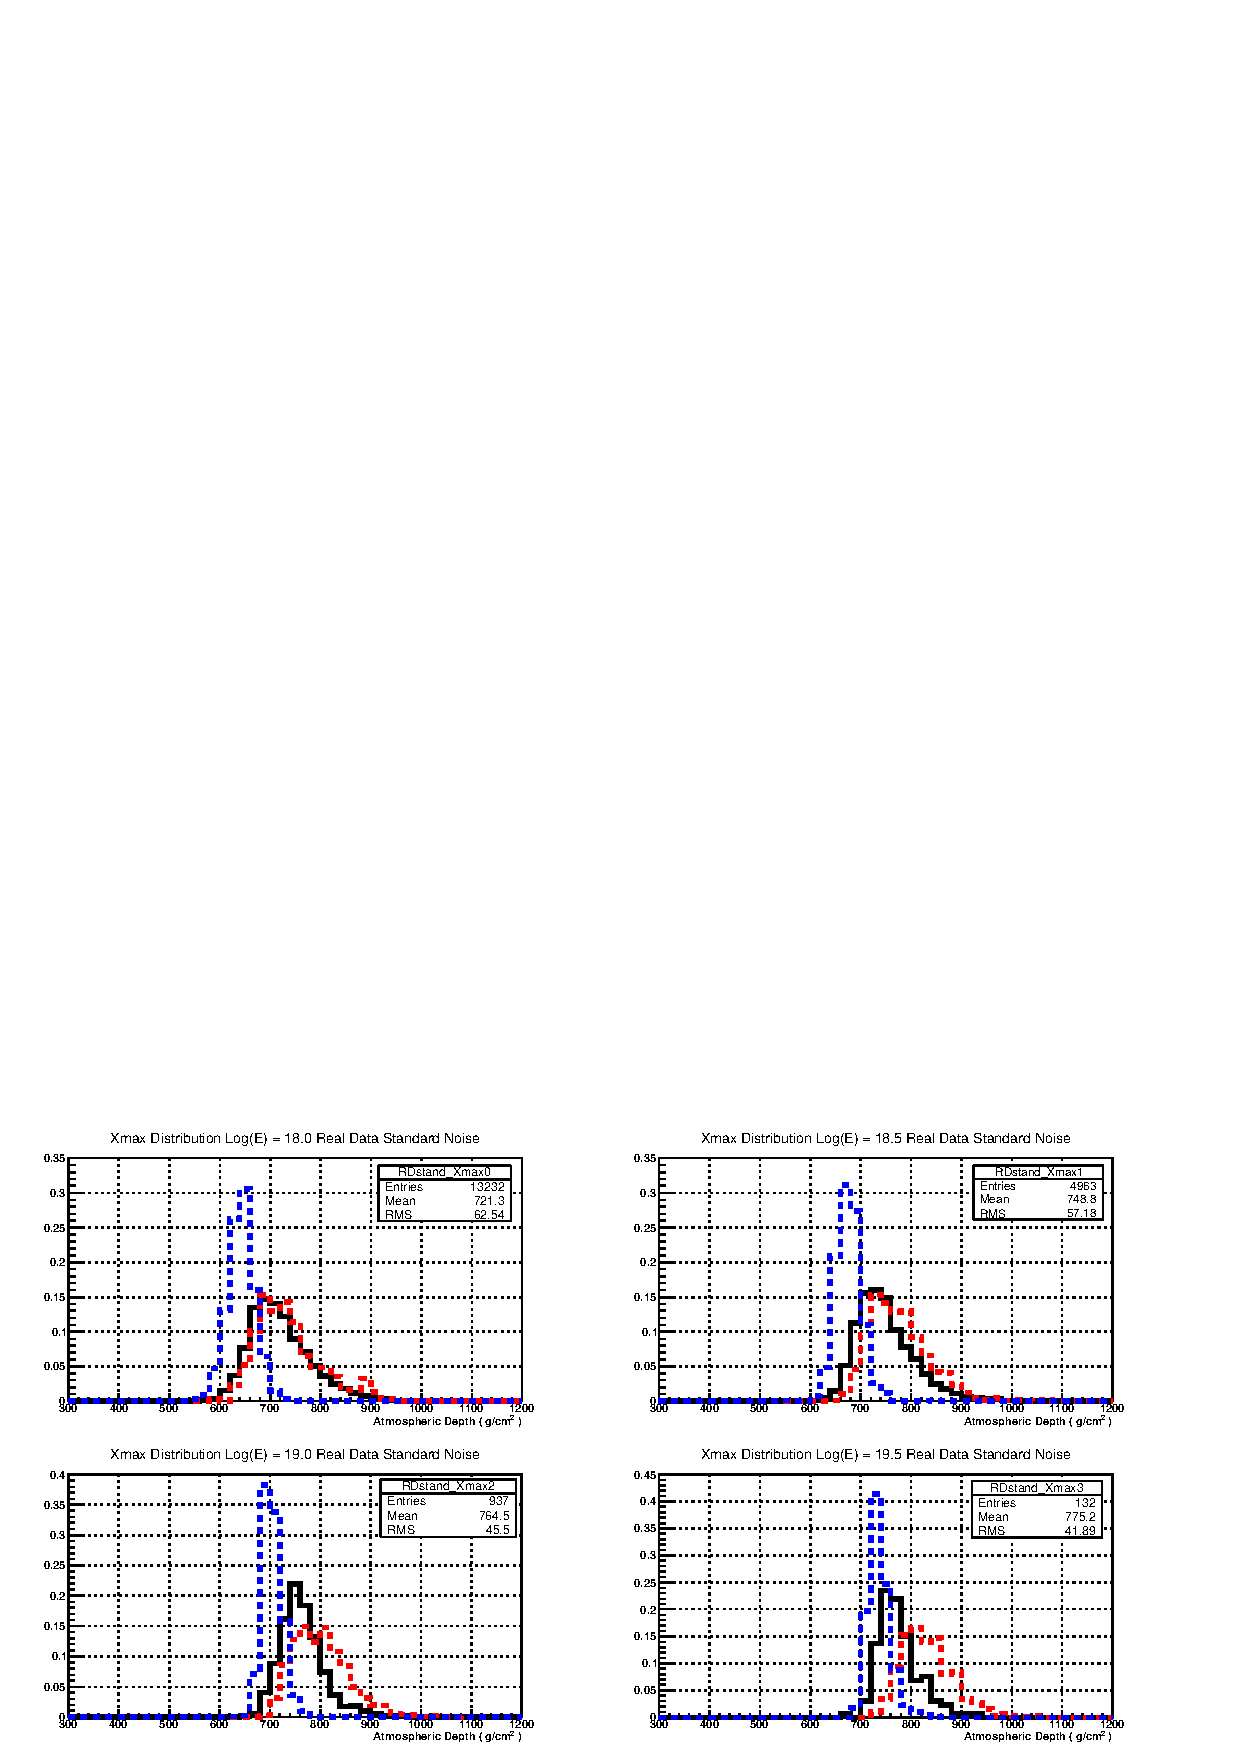
\includegraphics[width=\textwidth]{chapters/graphs/SelectionEff/RealDataAndSim_XmaxDistComp.pdf}
\caption{Distribution of Xmax with Real Data and simulation of proton and iron showers.}
\vspace{3mm}
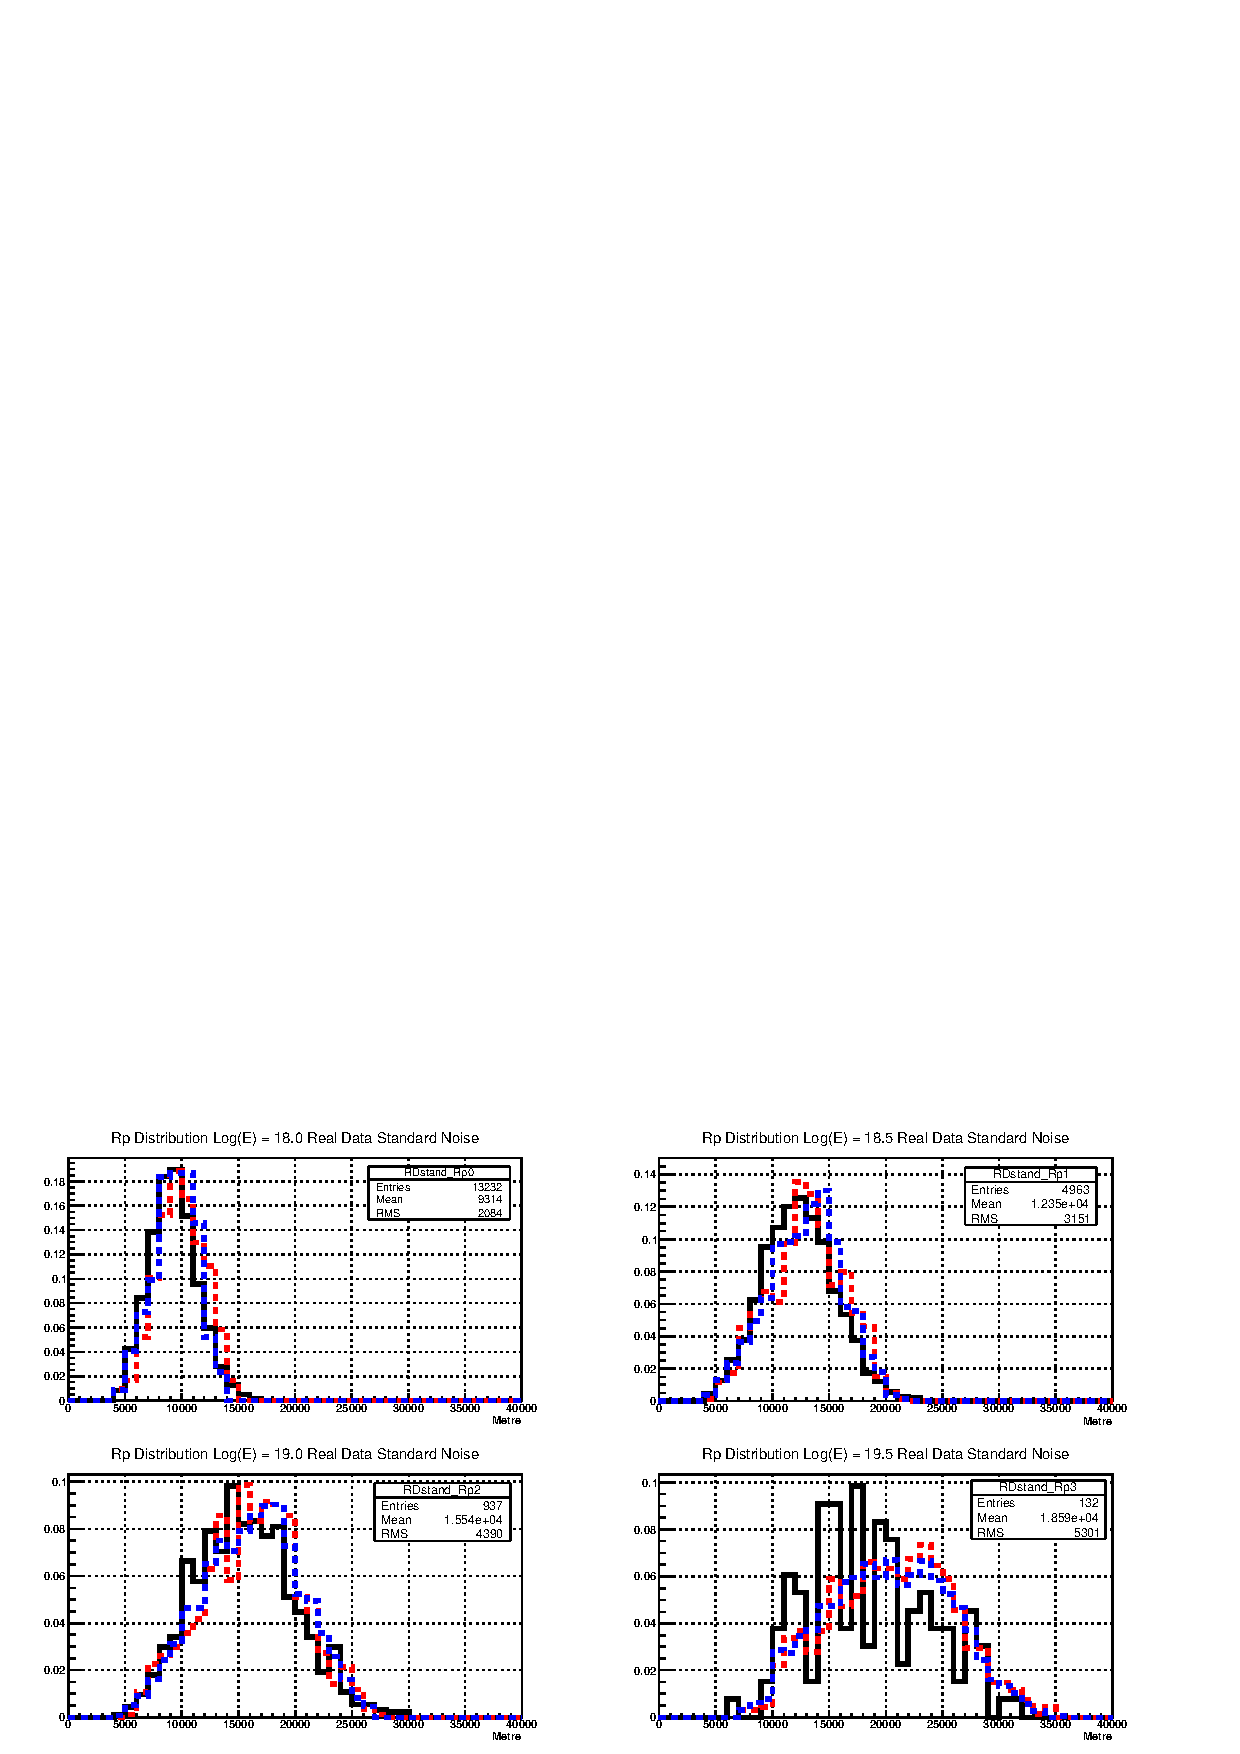
\includegraphics[width=\textwidth]{chapters/graphs/SelectionEff/RealDataAndSim_RpDistComp.pdf}
\caption{Distribution of Rp with Real Data and simulation of proton and iron showers.}
\end{figure}

\begin{figure}
\centering
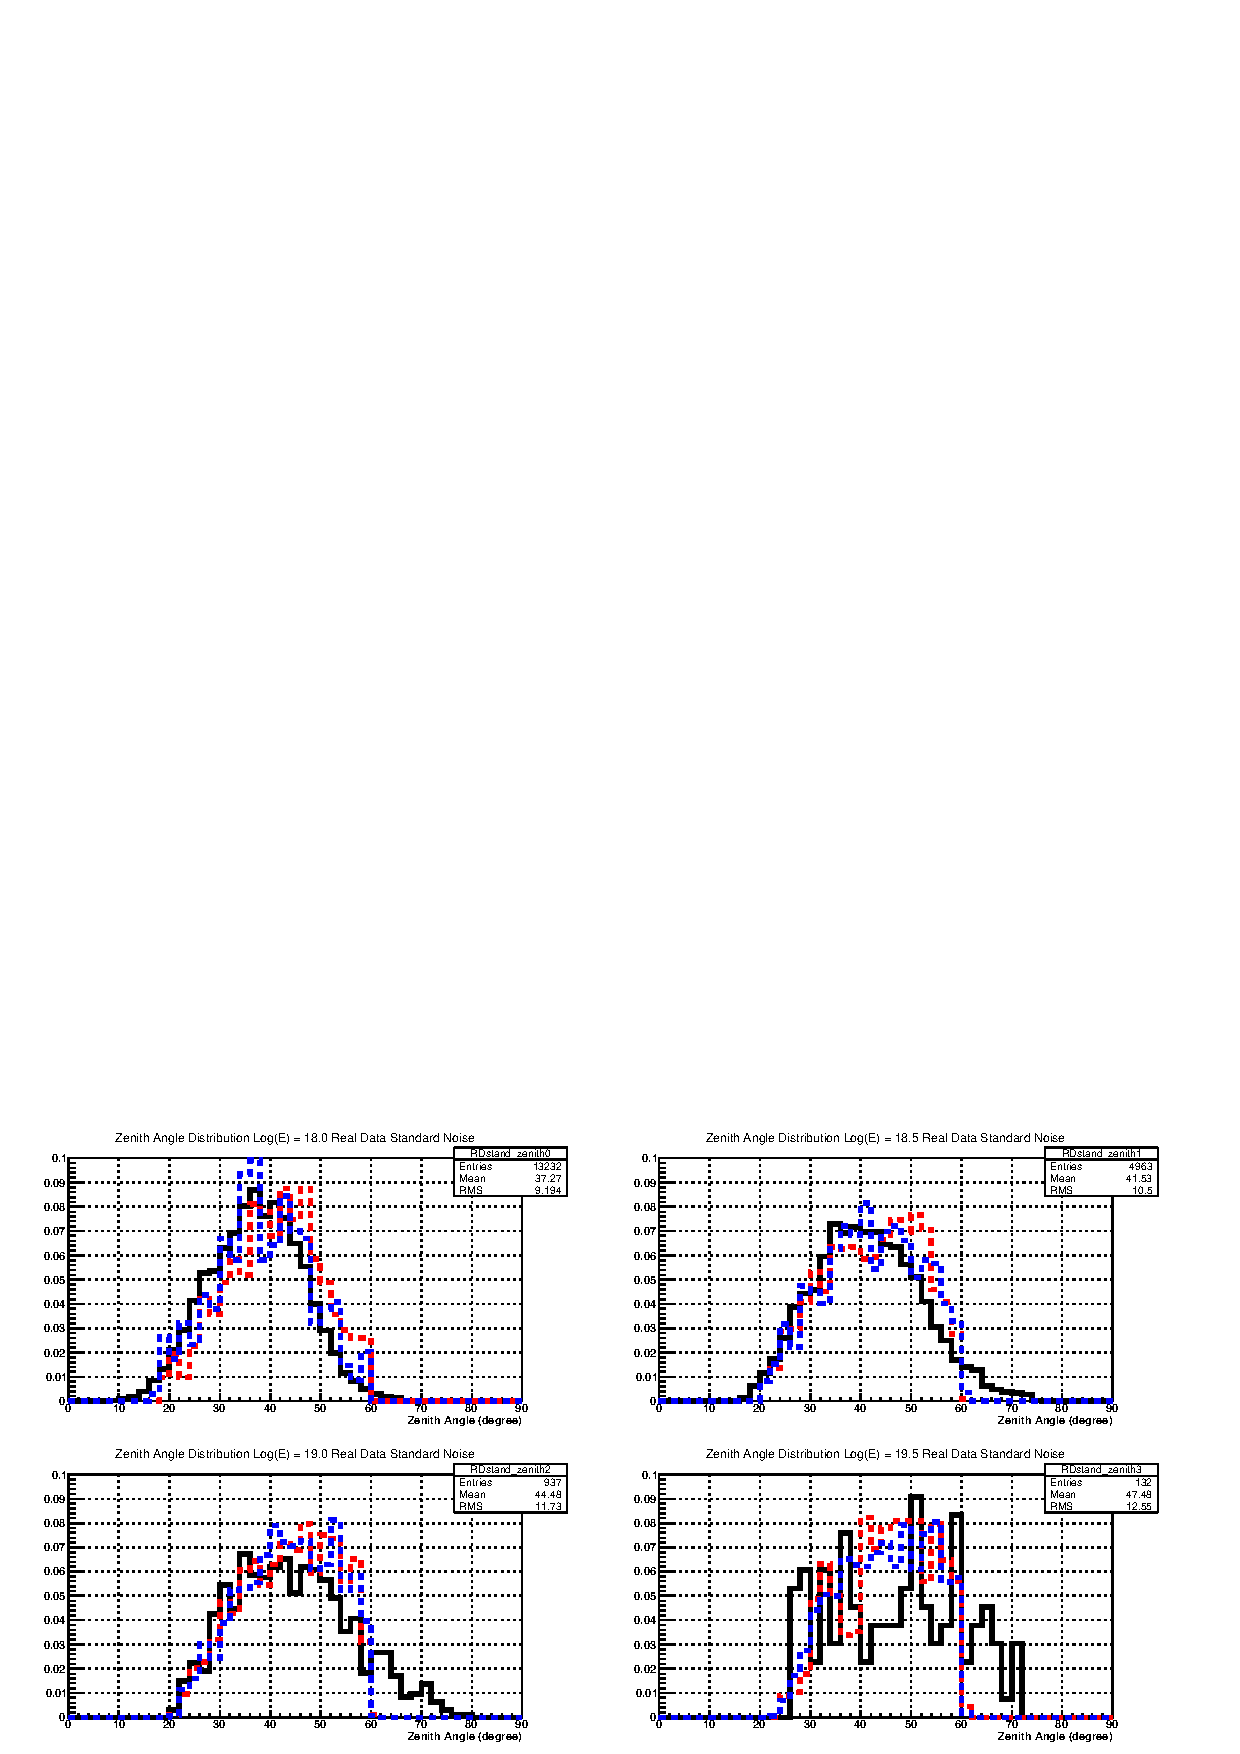
\includegraphics[width=\textwidth]{chapters/graphs/SelectionEff/RealDataAndSim_ZenithDistComp.pdf}
\caption{Distribution of Zenith angle with Real Data and simulation of proton and iron showers.}
\vspace{3mm}
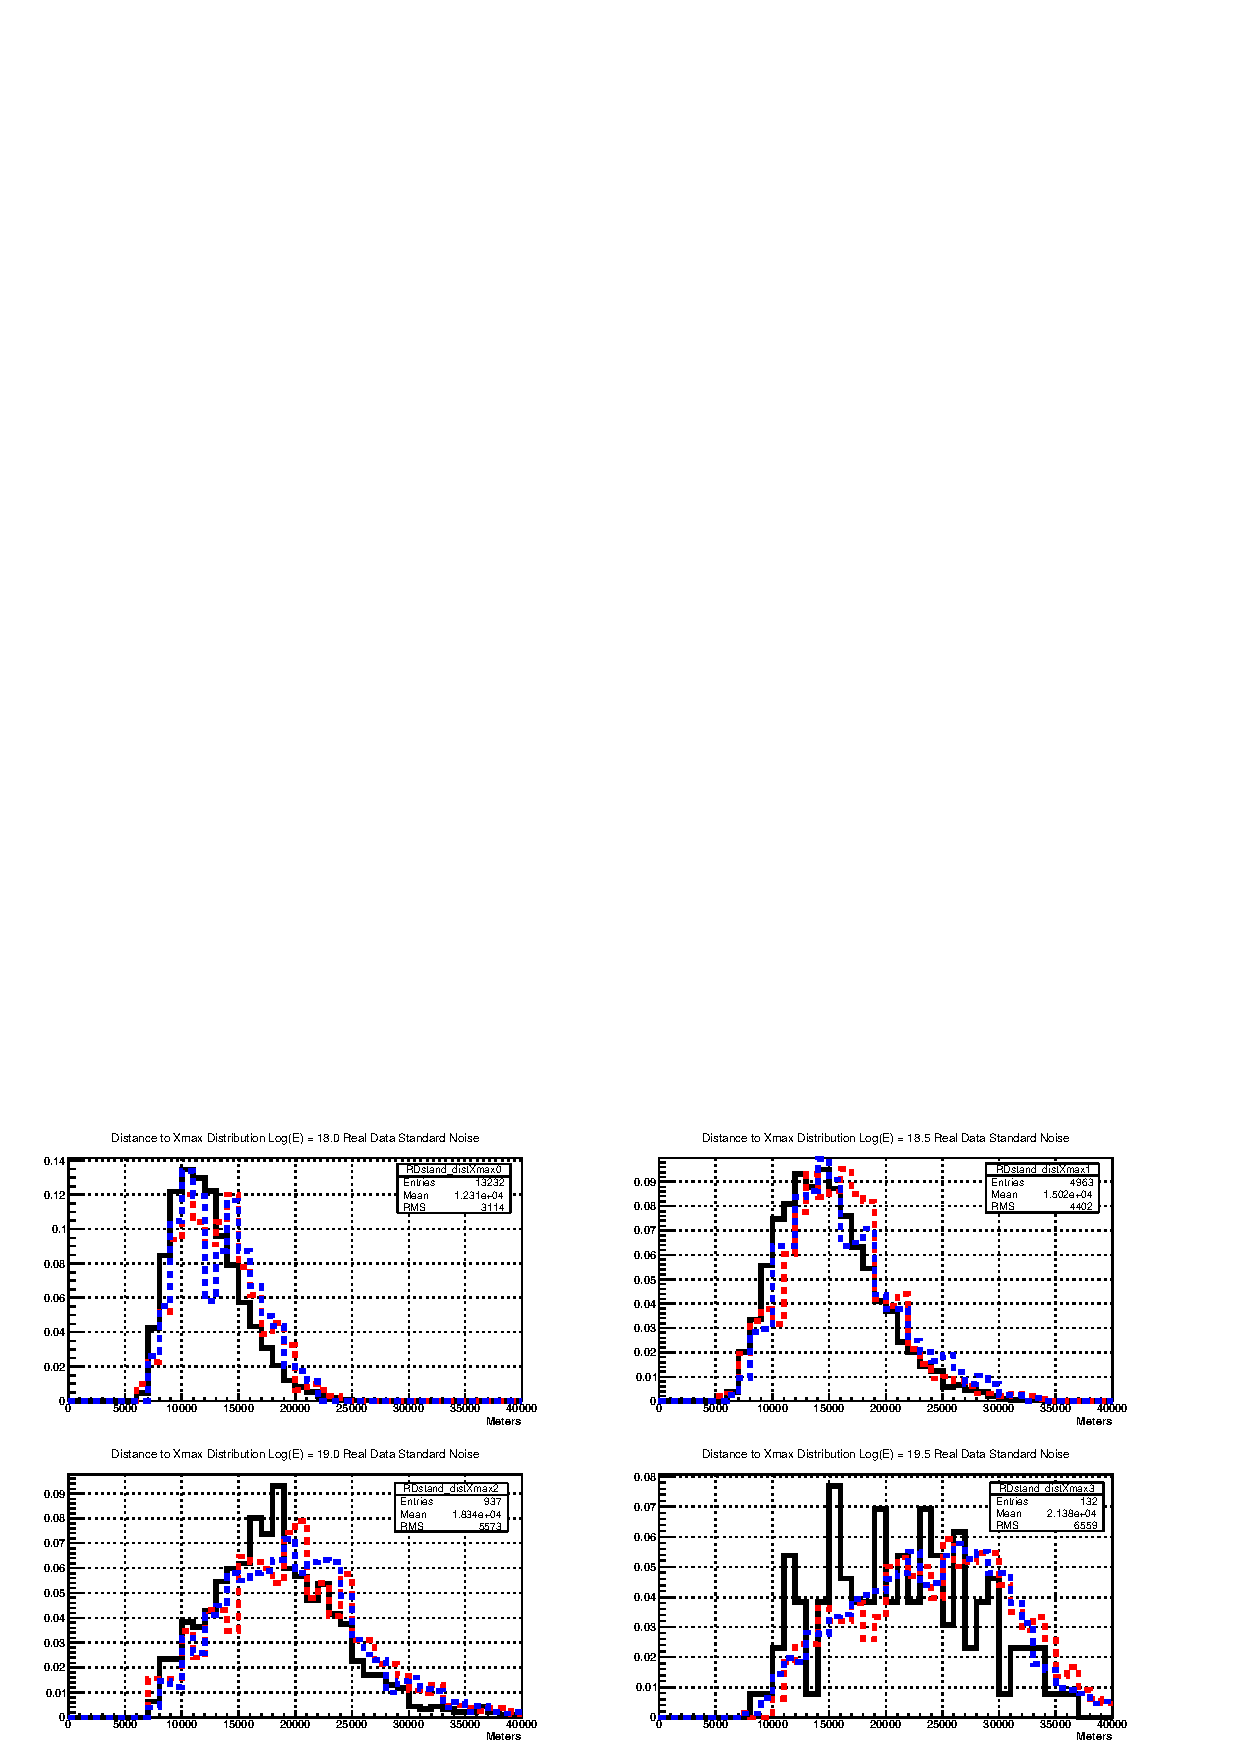
\includegraphics[width=\textwidth]{chapters/graphs/SelectionEff/RealDataAndSim_DistToXmaxDistComp.pdf}
\caption{Distribution of Distance to Xmax with Real Data and simulation of proton and iron showers.}
\end{figure}

\subsection{Results}
\begin{figure}
\centering
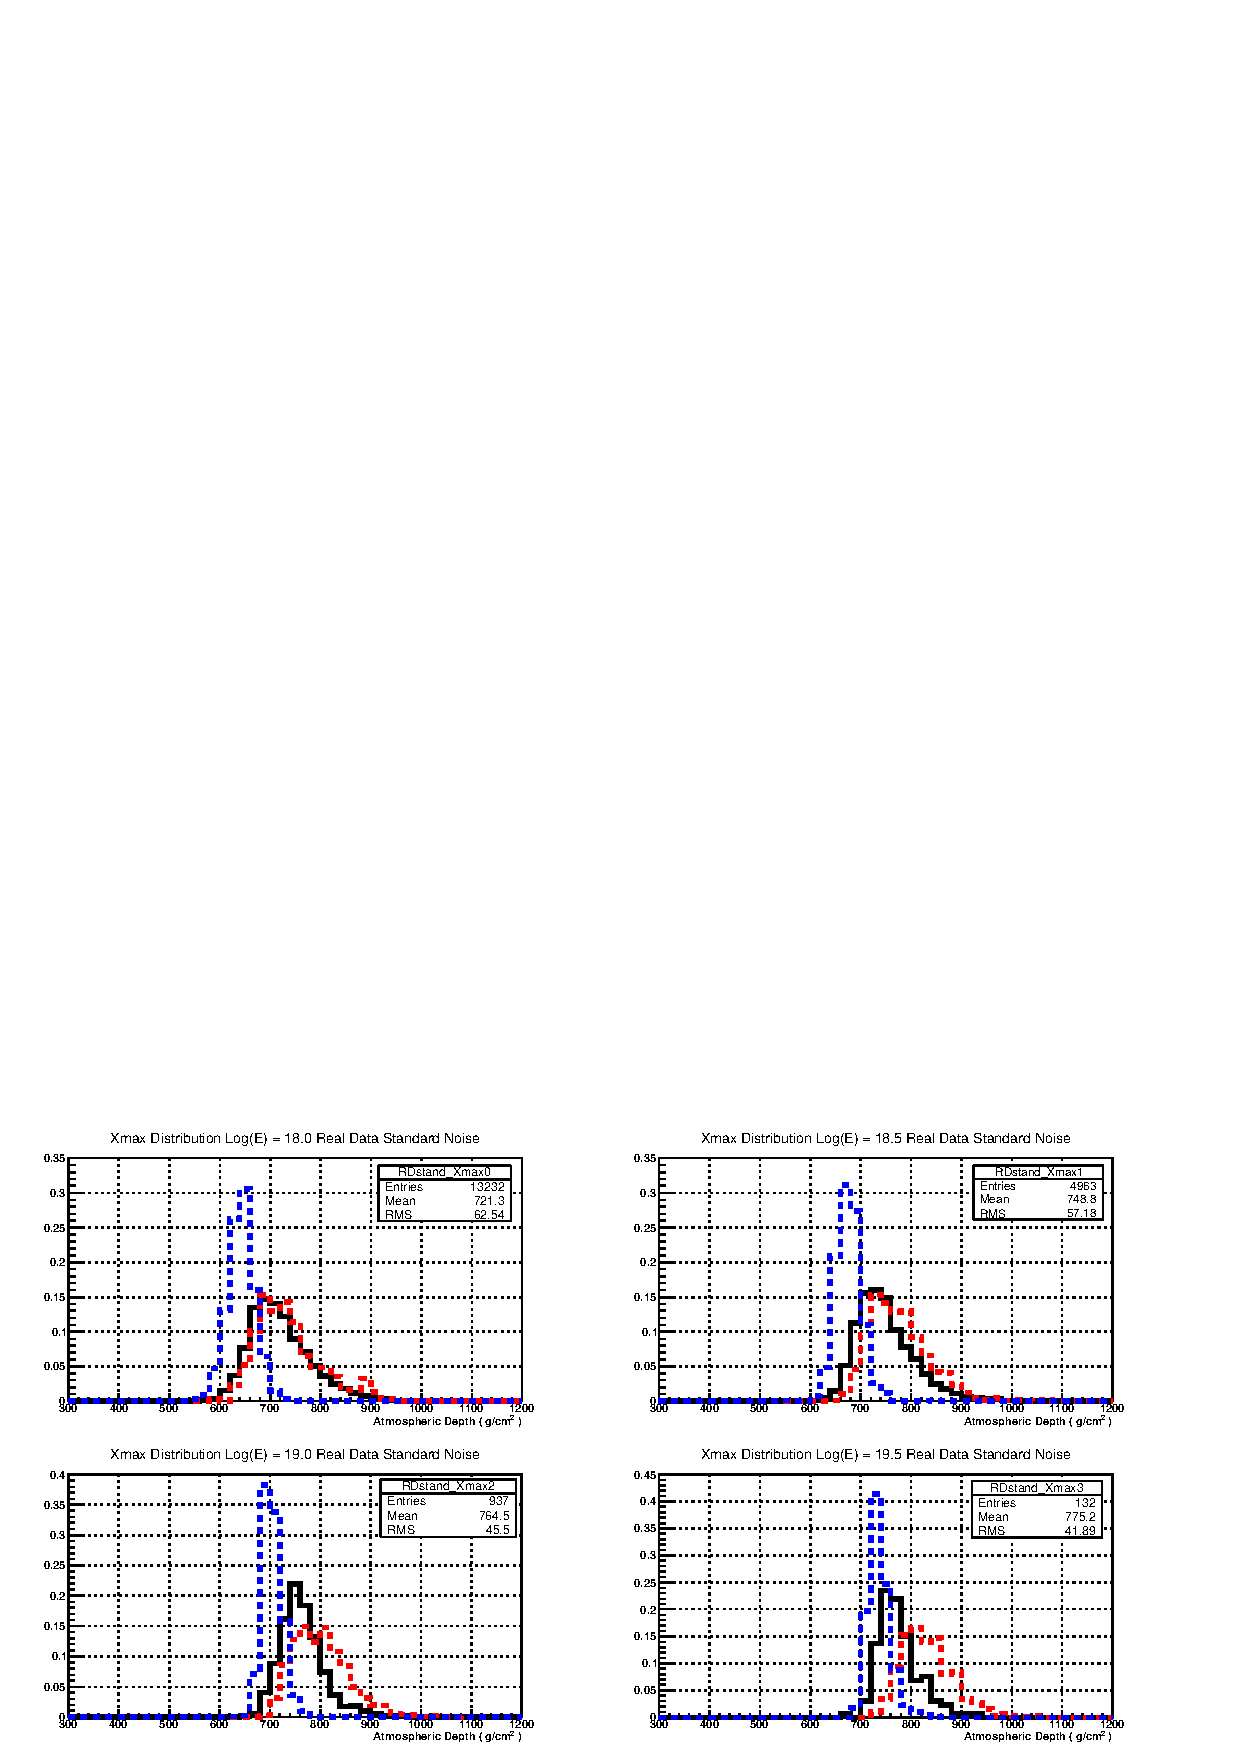
\includegraphics[width=\textwidth]{chapters/graphs/SelectionEff/RealDataAndSim_XmaxDistComp.pdf}
\caption{Distribution of Xmax with Real Data and simulation of proton and iron showers.}
\vspace{3mm}
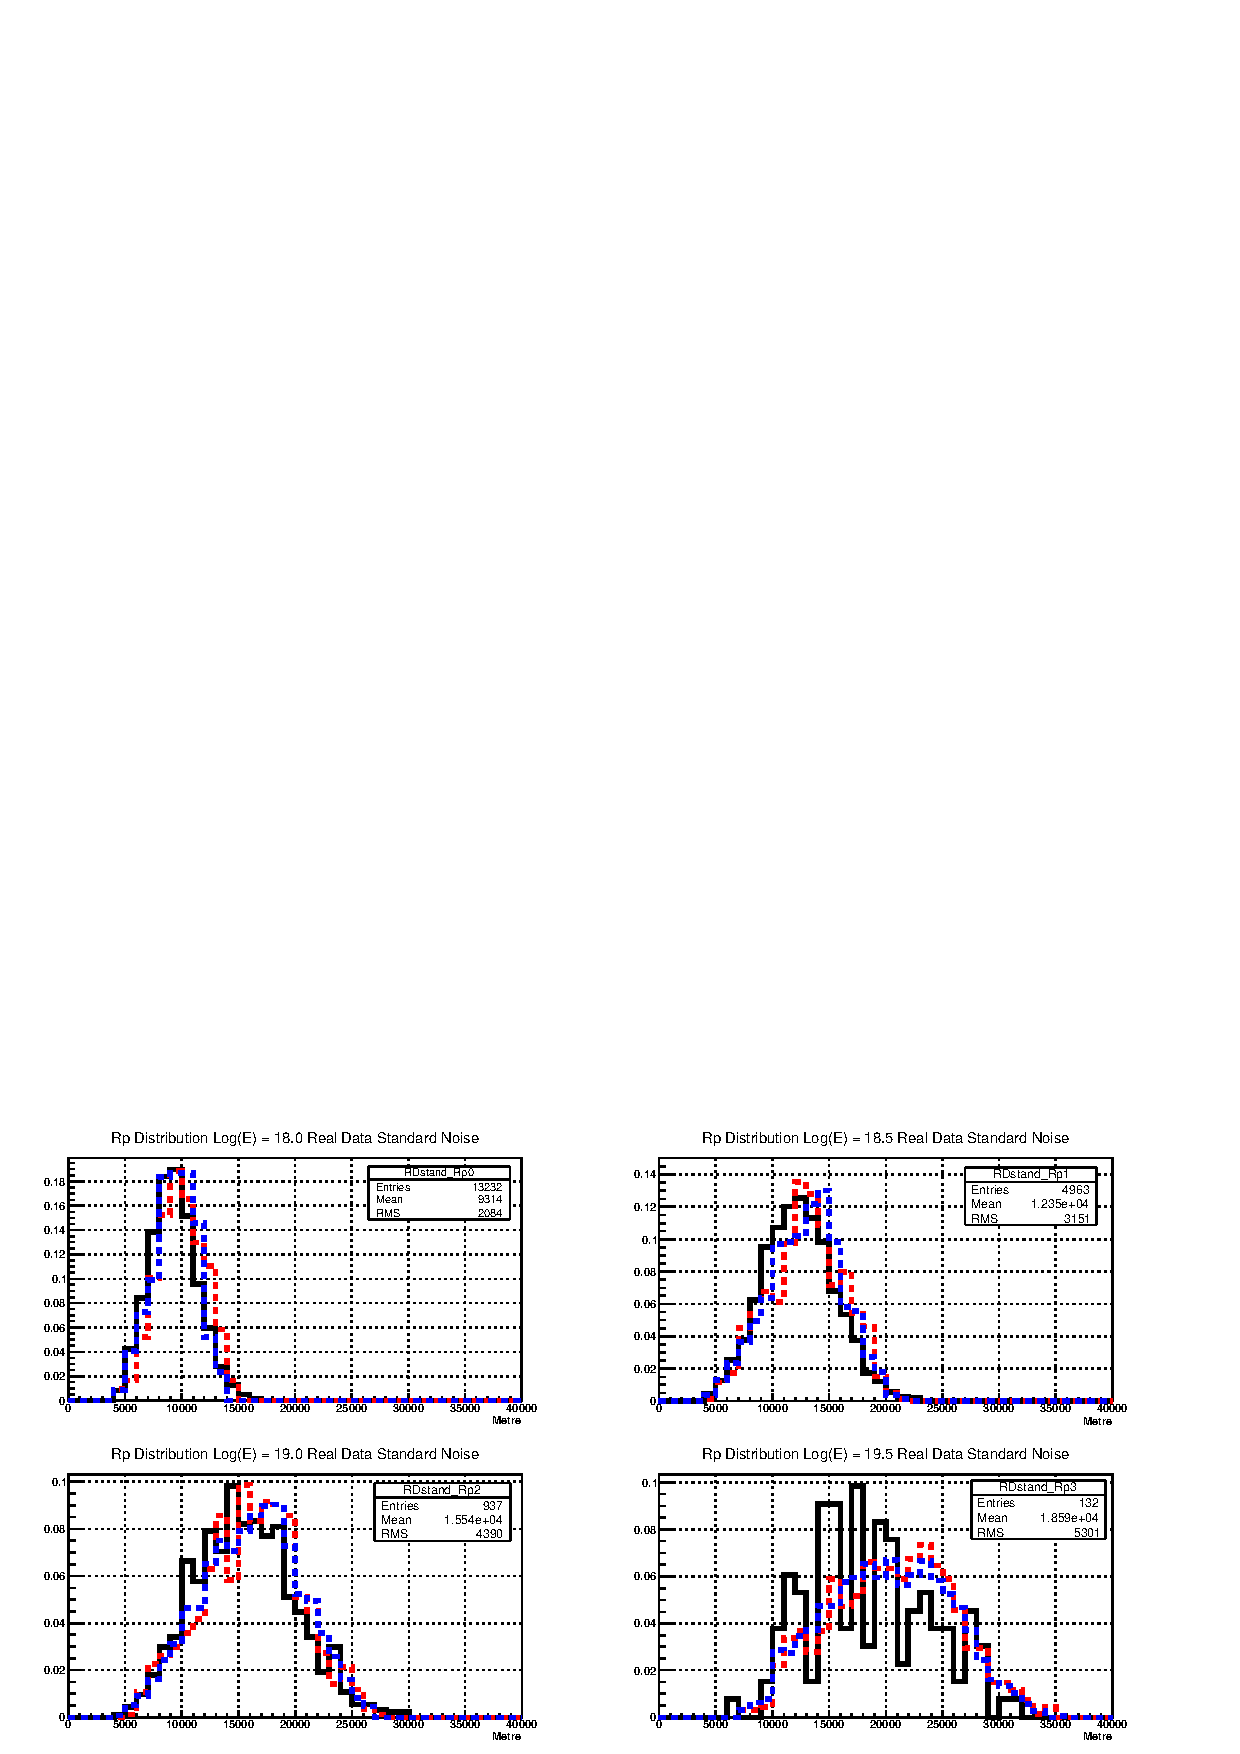
\includegraphics[width=\textwidth]{chapters/graphs/SelectionEff/RealDataAndSim_RpDistComp.pdf}
\caption{Distribution of Rp with Real Data and simulation of proton and iron showers.}
\end{figure}

\begin{figure}
\centering
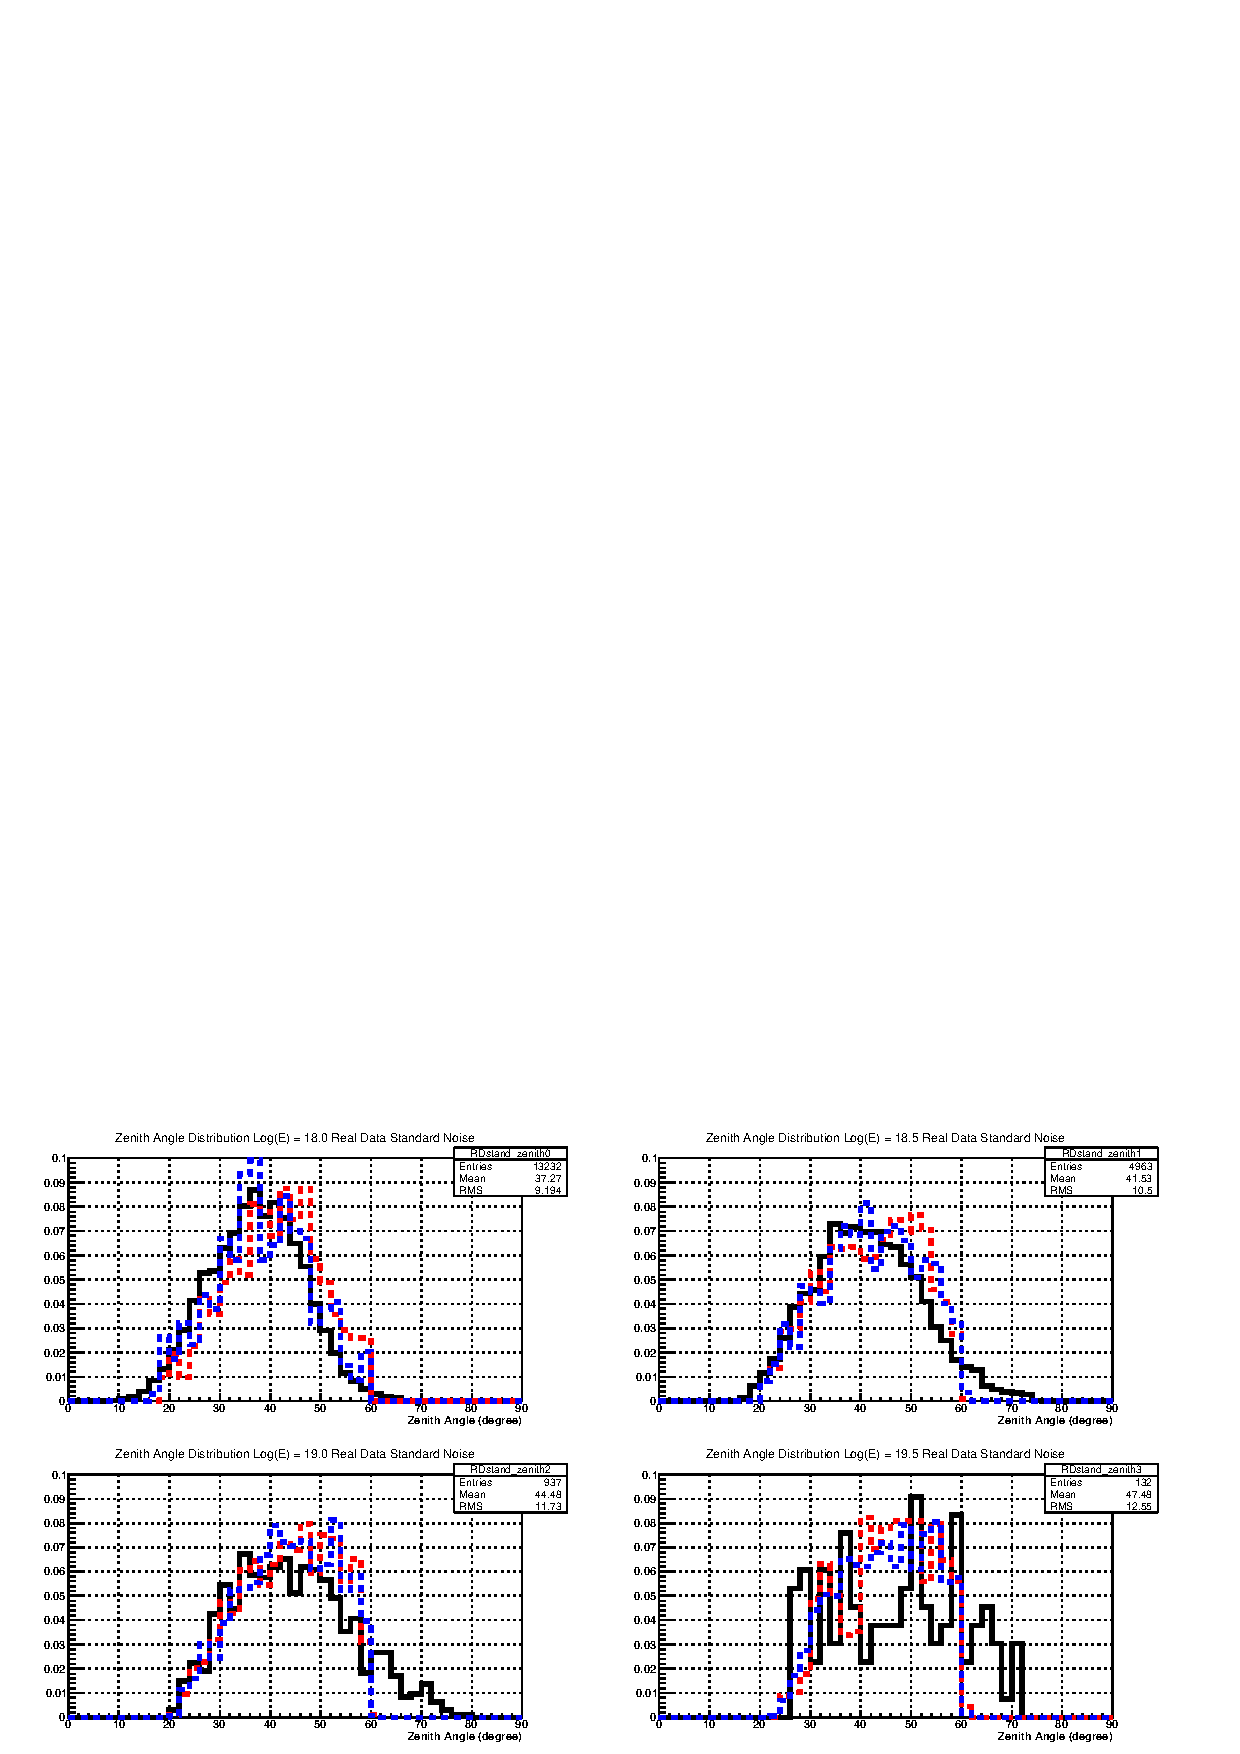
\includegraphics[width=\textwidth]{chapters/graphs/SelectionEff/RealDataAndSim_ZenithDistComp.pdf}
\caption{Distribution of Zenith angle with Real Data and simulation of proton and iron showers.}
\vspace{3mm}
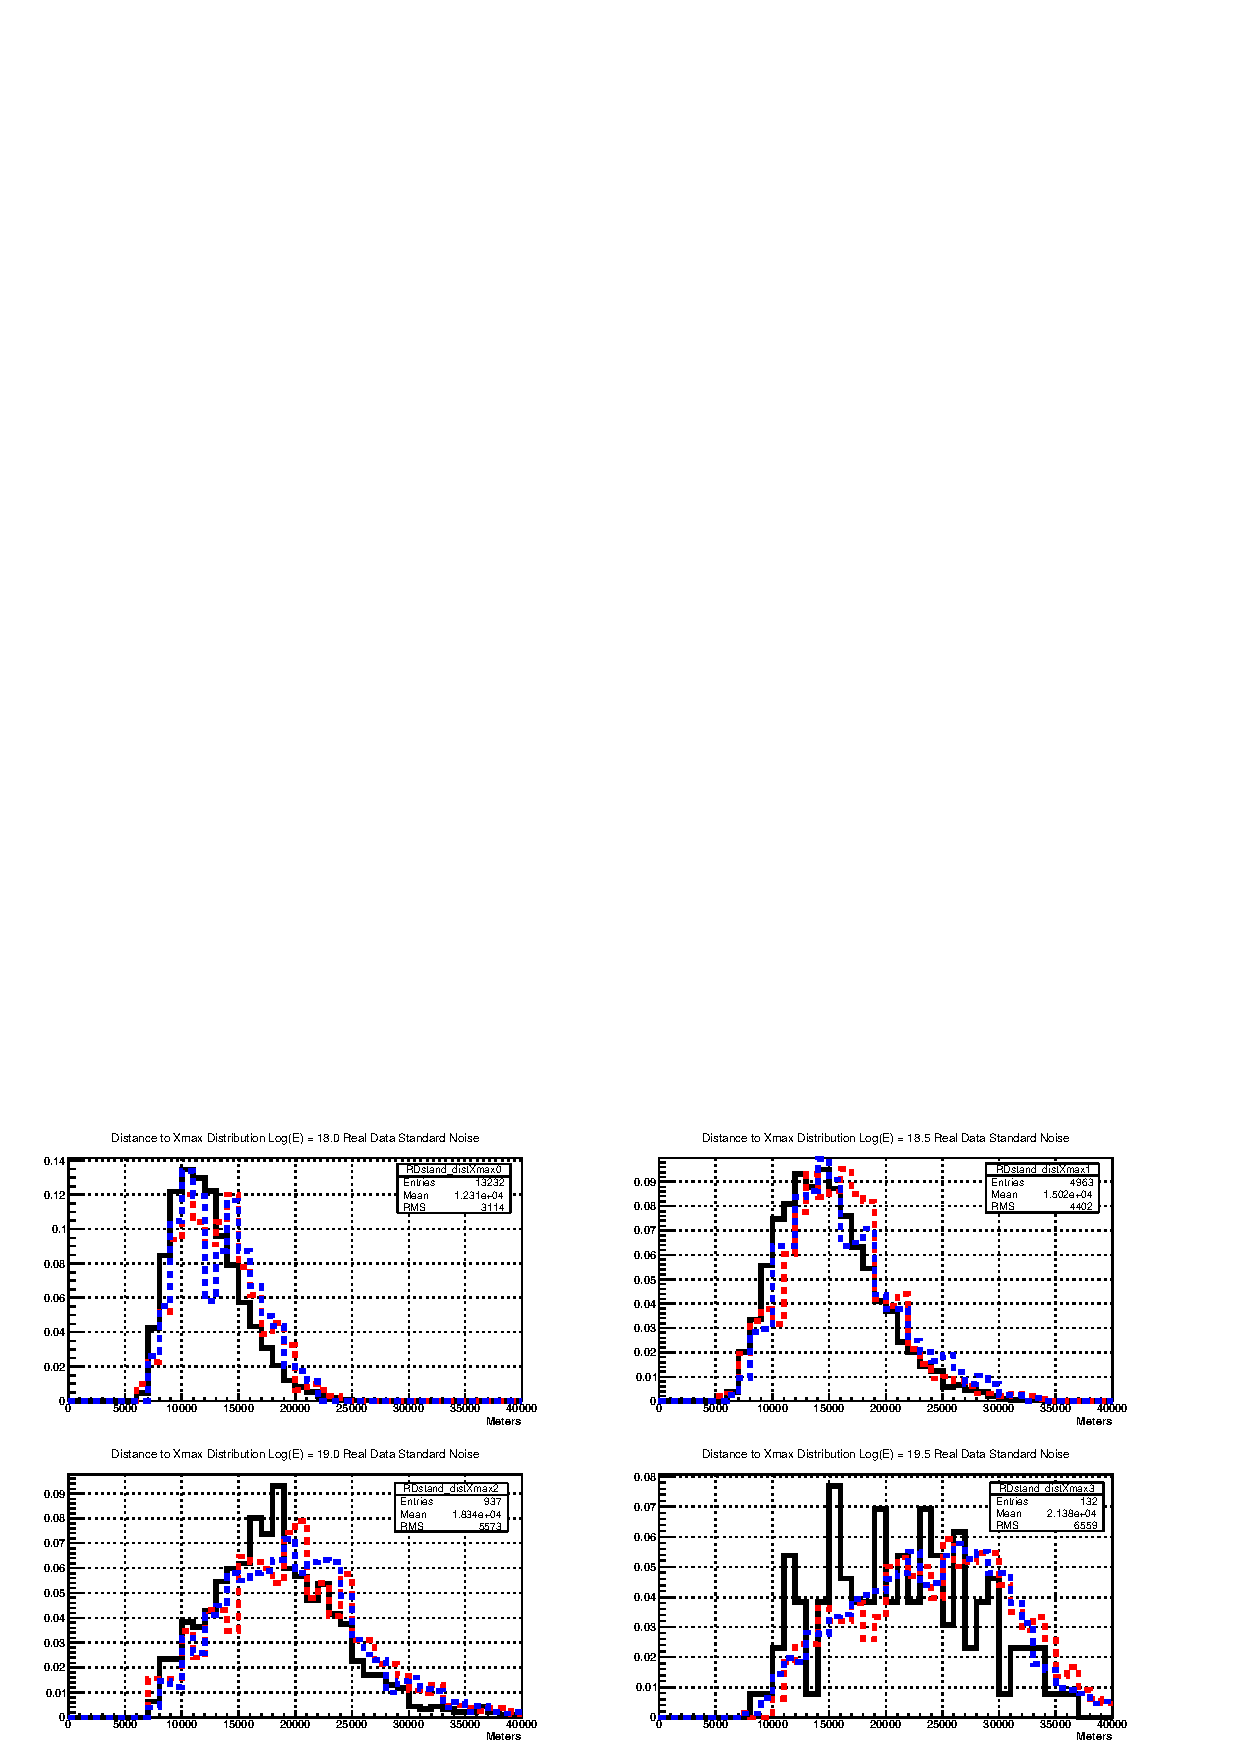
\includegraphics[width=\textwidth]{chapters/graphs/SelectionEff/RealDataAndSim_DistToXmaxDistComp.pdf}
\caption{Distribution of Distance to Xmax with Real Data and simulation of proton and iron showers.}
\end{figure}


\begin{figure}
\centering
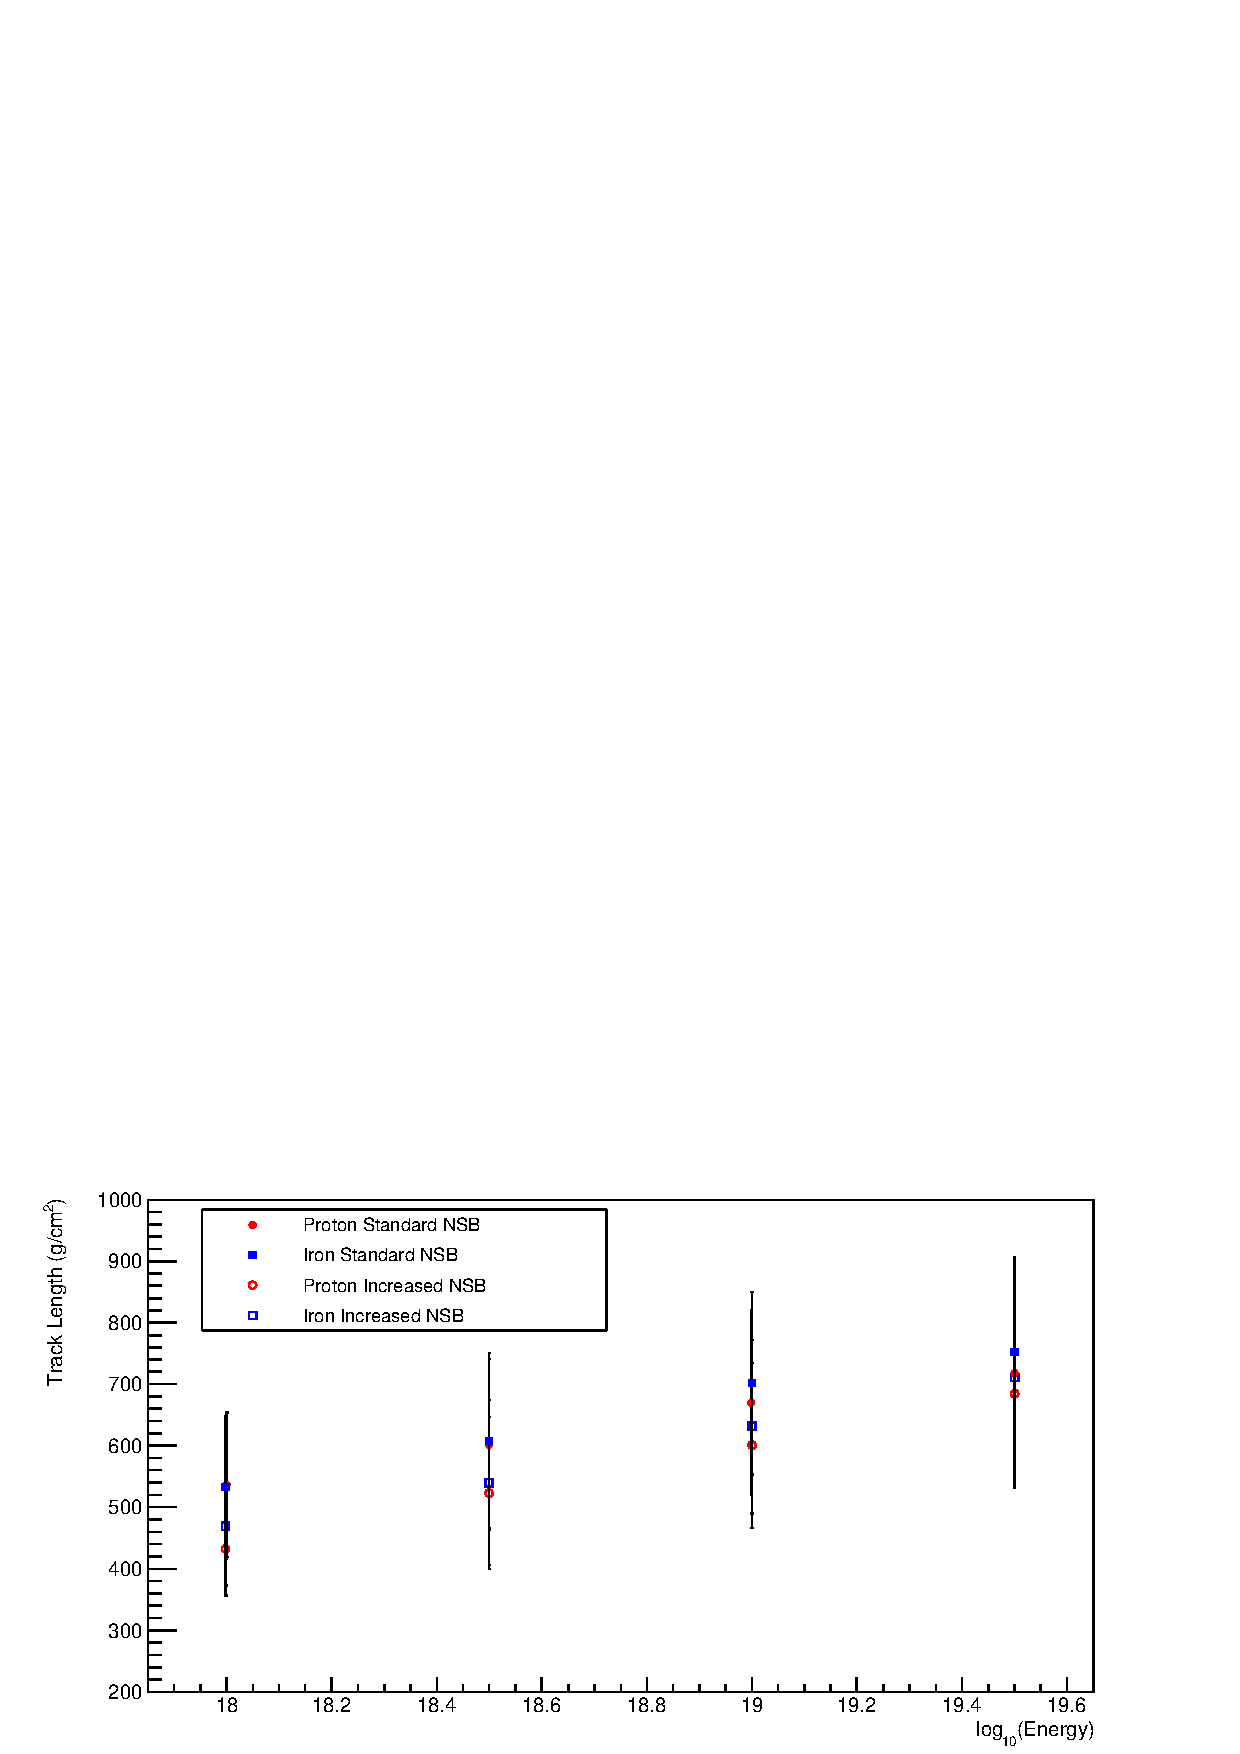
\includegraphics[width=\textwidth]{chapters/graphs/SelectionEff/Simulation_TrackLength_Comb_StandANdIncreasedNSB.pdf}
\caption{Track length using simulation of proton and iron CONEX showers.} \label{fig:TrackLength_Sim}
\end{figure}
\subsection{Discussion}

\section{Conclusion/Summary}